% Chapter Template

\chapter{The Coupled Cluster Method} % Main chapter title

\label{Chapter5} % Change X to a consecutive number; for referencing this chapter elsewhere, use \ref{ChapterX}

\lhead{Chapter 6. \emph{The Coupled Cluster Method}} % Change X to a consecutive number; this is for the header on each page - perhaps a shortened title

%----------------------------------------------------------------------------------------
%	Introduction
%----------------------------------------------------------------------------------------

\section{Historical Account}


As is the case with many contributions to science, it is hard to
pinpoint the origin of the Coupled Cluster methods to one single
scientific work. It is however commonly accepted that the groundbreaking
work was made by the nuclear physicists Fritz Coester and
Hermann Kümmel in the mid and late 50s. At this time the computational aspects
of many body theory was still in its early infancy, although some
variational Hartree-Fock calculations had been performed in the
quantum chemistry community. \cite{Kummel}

One important discovery that may have motivated work on the Coupled
Cluster method was made by J. Hubbard, who laboriously inspected the
time independent perturbation series to all orders and found that only
linked terms contribute to the energy, as well as that the energy
associated with these terms was \emph{extensive} \cite{Hubbard}.

Coester was then shortly after the work of Hubbard able to derive
basically the same results using the \emph{exponential ansatz} and
\emph{the Hausdorff expansion} \cite{Kummel}. In the following years,
Kümmel and Coester published a number of papers describing the method \cite{Coester1958, Coester1960b},
and by the late 1950s the method was well understood \cite{Kummel}.

Together with Haag, Coester was also able to show that the
exponential ansatz was a natural choice for the system's wave function
\cite{Coester1960a}, meaning that the choice was not as arbitrary as one may get
the impression of when reading modern books on the
subject \cite{ShavittBartlett2009}.


Despite this, it was not until 1966 that the first real applications
of the method were made, and these were made by the quantum chemist Jiri
Cizek \cite{Cizek1966}. Coupled Cluster calculations for nuclear
matter were performed in the late 1970s and early 1980s \cite{kummel1978,day1981}.

Today, the so called Hartree-Fock + CCSD(T) (Coupled Cluster Singles
Doubles and Perturbative Triples) calculation is considered the "gold
standard" of quantum chemistry, due to its relatively low
computational cost compared to its ability to account for important
correlations in many systems.


\section{The exponential ansatz}
The derivation of the coupled cluster method begins with assuming that
the operator that brings the reference state into the true system
state can be represented by the exponetial operator
\begin{equation}
e^{\hat{T}} ,
\label{eqn:exponential_ansatz}
\end{equation}
where the \emph{cluster operator} is defined as
\begin{equation}
\hat{T} \equiv  \hat{T}_1 + \hat{T_2} + ... = 1 + \sum_{ai} t_i^a a_{a}^\dagger a_i + \sum_{ai} t_{ij}^{ab} a_{a}^\dagger a_{b}^\dagger a_i a_j + ...
\end{equation}

As may be seen from the second quantized form of the cluster operator,
its terms will cause an excitation of the reference state. For
example, the excitation operator $\hat{T}_1$ generates  a singly
excited reference state
\begin{equation}
\hat{T}_1\vert \Phi_0\rangle = \sum_{ai} t_i^a a_{a}^\dagger a_i|\Phi_0\rangle = \sum_{ai} t_i^a \vert \Phi_i^a\rangle,
\end{equation}
while the $\hat{T}_2$ operator creates a doubly excited reference state
\begin{equation}
\hat{T}_2 \vert \Phi_0\rangle = \sum_{abij} t_{ij}^{ab} a_{a}^\dagger a_{b}^\dagger a_i a_j|\Phi_0\rangle = \sum_{abij} t_{ij}^{ab} \vert \Phi_{ij}^{ab}\rangle,
\end{equation}
and so on. 

For reasons that will become clear shortly, there is no need to
include excitation operators beyond $\hat{T}_4$ for systems containing at most two body interactions. Truncations in the cluster operator are commonly made to give rise to the different
types of coupled cluster methods.

The coefficients $t^{ab..}_{ij...}$ are commonly referred to as \emph{amplitudes}, and they are the quantities we seek. 

As for any exponential function, we may expand it as
\begin{equation}
e^{\hat{T}} = 1 + \hat{T} + \frac{1}{2!} \hat{T}^2 + \frac{1}{3!} \hat{T}^3 + ... ,
\end{equation}
so the exponential ansatz may be written
\begin{equation}
e^{\hat{T}}  \vert \Psi_0 \rangle = (1 + \hat{T} + \frac{1}{2!} \hat{T}^2 + \frac{1}{3!} \hat{T}^3 + ...) \vert \Psi_0 \rangle .
\end{equation}

\section{Size consistency}
The concept of size consistency was introduced by Pople {\em et al.} in 1978
\cite{Pople} to describe methods that properly represent systems in
the noninteracting limit. A system of electrons interacting through
the Coulomb force has a noninteracting limit when the distance
between the electrons is so large that the energy of this
configuration should correspond to the energy of an equal number of
noninteracting electrons.

In other words, a size consistent method should for the interacting
systems A and B produce energy calculations in the noninteracting
limit where \cite[p.12]{ShavittBartlett2009}
\begin{equation}
E(AB) = E(A) + E(B)
\end{equation}

Because of the fundamental assumption of pairing of electrons in the
restricted Hartree-Fock (RHF) method, this method is not size consistent for
systems such as the $H_2$ molecule. This shortcoming may however be
mended by performing a coupled cluster calculation on top of the RHF,
producing size consistent energies when gradually separating the
hydrogen nucleis (and their electrons). This is illustrated by a
comparison of RHF, unrestricted Hartree-Fock (UHF) and RHF+CCSD (coupled cluster theory at the level of singles and doubles excitations only) 
for the $H_2$ molecule in Fig.
\ref{fig:uhf_rhf_ccsd_h2}. It is clear that since the RHF method forces the
electrons of each hydrogen atom to pair, the energy is wrongly estimated
compared to the exact energy as we separate the H nuclei. 

By performing a CCSD calculation employing  the RHF basis, this restriction is lifted, allowing the
electrons to fall into their natural orbits. An unrestricted Hartree-Fock calculation on the other hand does
not assume the electrons to be paired, allowing thereby for a natural
behavior as the separation in distance between the two H nuclei increases.


\begin{figure}[p]
    \centering
    \includegraphics[width=0.8\textwidth]{uhf_rhf_ccsd_h2}
    \caption{Comparison of UHF, RHF and RHF+CCSD for a $H_2$
      molecule. These results were produced by the author using a self-developed 
      solver \cite{FermionMingle} that utilizes gaussian
      basis sets to enable RHF, UHF, CCD and CCSD calculation on atoms
      and molecules. These results
      illustrate the size consistency of the CCSD equations, and
      the lack of size consistency in the RHF case. (The vertical
      jumps in the curves are regions where the solver failed to
      converge due to improperly chosen relaxation parameters. Central parts of the code \cite{FermionMingle} that was used to produce these calculations was developed by the author as part of another course.)}
    \label{fig:uhf_rhf_ccsd_h2}
\end{figure}


When comparing CC with CI, we will find that the $\hat{C}_2$ operator
has a corresponding combination of cluster operators
\begin{equation}
\hat{C}_2 = \hat{T}_2 + \frac{1}{2}(\hat{T}_1)^2.
\end{equation} 
The last quadratic term above is commonly referred to as a
\emph{disconnected cluster}, and such terms are responsible for
ensuring the consistency of the CC method.



\section{Extensivity}

A related concept to consistency is \emph{size extensivity}, as
introduced by Bartlett \cite{Bartlett1981}. A quantum mechanical model
may be called \emph{extensive} if the energy of this model scales
correctly with the size of the
system \cite[p.11]{ShavittBartlett2009}. This is analogous to
extensive properties in statistical mechancial systems, that scales
linearly with the size of the system \cite[p.9]{Linder}.

When performing calculations on periodic systems such as gases or
solids, extensivity is a feature that allows us to extrapolate results
beyond the limits of the simulation cell.

For the coupled cluster method, extensivity is an inherent property of
the exponential ansatz (see Eq. (\ref{eqn:exponential_ansatz})). This may be shown
by considering that the reference state is separable, implying that
\begin{equation}
\phi_0(A,B) = \phi_0(A)\phi_0(B).
\end{equation}

Furthermore, the cluster operators are additive and we have
\begin{equation}
\hat{T}(A,B) = \hat{T}(A) + \hat{T}(B) .
\end{equation}

It then follows that the total wave function is multiplicatively separable
\begin{equation}
\Psi(A,B) = e^{T(A) + T(B)}\phi_0(A,B) = e^{T(A)}\phi_0(A)e^{T(B)}\phi_0(B).
\end{equation}

Thus, the energy is additive:
\begin{equation}
\hat{H}(A,B)\Psi(A,B) = [E(A) + E(B)]\Psi(A,B).
\end{equation}


\section{Deriving the coupled cluster equations}

We will derive the coupled cluster equations in four steps. First we
shall do some more work on the exponential ansatz to derive a form
that is more easily translated to actual calculations, secondly we
will introduce diagrammatic rules that will simplify derivations
considerably, and then we shall briefly comment upon how to translate
these rules into a code that makes the process of deriving coupled
cluster equations (and code) of any order remarkably simple.

Since the actual equations that are worked into a high-performance code
will depend upon how we truncate the ansatz, we will then finally
derive the full equations using the above mentioned code in increasing
order of complexity.

\section{Unwrapping the exponential ansatz}

\subsection{The CC effective Hamiltonian}

The actual quantity we seek is the correlation energy $\Delta e$ as
found by solving the Schrödinger equation for the exponential ansatz
and the normal ordered Hamiltonian Eq.~(\ref{eqn:hamiltonian_N})
\begin{equation}
\hat{H}_N e^{\hat{T}} \vert \Phi_0 \rangle =  \Delta e  e^{\hat{T}} \vert \Phi_0 \rangle.
\end{equation}
We may reorganize this into
\begin{equation}
(\hat{H}_N - \Delta e) e^{\hat{T}} \vert \Phi_0 \rangle = 0.
\end{equation}
By multiplying with the inverse exponential, we find
\begin{equation}
(e^{\hat{-T}} \hat{H}_N e^{\hat{T}} - \Delta e)  \vert \Psi_0 \rangle = 0,
\label{eqn:cc1}
\end{equation}
where the non-Hermitean operator
\begin{equation}
e^{\hat{-T}} \hat{H}_N e^{\hat{T}}  \equiv \mathcal{H},
\end{equation}
is a similarity transformed Hamiltonian, often called the \emph{CC effective Hamiltonian}.

By projecting Eq.~(\ref{eqn:cc1}) onto the reference state, we may then solve for the correlation energy
\begin{equation}
\langle \Phi_0 \vert e^{\hat{-T}} \hat{H}_N e^{\hat{T}} \vert \Psi_0 \rangle = \Delta e.
\label{eqn:cc2}
\end{equation}

It also follows that
\begin{equation}
\langle \Phi^* \vert e^{\hat{-T}} \hat{H}_N e^{\hat{T}} \vert \Psi_0 \rangle = 0,
\label{eqn:cc2}
\end{equation}
where $\Phi^*$ represents any excited state. This last equation will aid us in solving the amplitudes.

\subsection{Non-variational coupled cluster}

At this point we should note that the CC effective Hamiltonian is no longer Hermitean, since
\begin{equation}
\mathcal{H}^\dagger = (e^{\hat{-T}} \hat{H}_N e^{\hat{T}})^\dagger = (e^{\hat{-T}})^\dagger \hat{H}_N (e^{\hat{T}})^\dagger = (e^{\hat{-T^\dagger}}) \hat{H}_N (e^{\hat{T^\dagger}}) \neq \mathcal{H}
\end{equation}

A consequence is that truncations in the cluster operator will cause
the energy expression in Eq. (\ref{eqn:cc2}) to no longer be
variational, and thus the energy does no longer represent an upper
bound to the ground state energy \cite{CrawfordSchaefer}. In practice,
however, solving the resulting equations obtained from the
projection technique in Eq. (\ref{eqn:cc2}) will still provide us
with an energy close to the real expectation value even for truncated
cluster operators \cite{CrawfordSchaefer}.

\subsection{The Hausdorff Expansion}

The Hausforff expansion (or Baker-Campbell-Hausdorff formula) provides
us with the means of rewriting the CC effective Hamiltonian in terms
of nested commutators \cite[p.293]{ShavittBartlett2009}:
\begin{equation}
\mathcal{H} = \hat{H}_N + [\hat{H}_N, \hat{T}] + \frac{1}{2} [[\hat{H}_N, \hat{T}], \hat{T}] +  \frac{1}{3!} [[[\hat{H}_N, \hat{T}], \hat{T}], \hat{T}] + \frac{1}{4!} [[[[\hat{H}_N, \hat{T}], \hat{T}], \hat{T}], \hat{T}].
\end{equation}

The reason that this sum of nested operators truncates at the
four-fold commutator, will become apparent if we use Wicks generalized
theorem to evaluate the expansion. For two strings of evenly numbered
creation- and annihilation operators, we will find the commutator
\begin{equation}
[A,B] = AB - BA = np[A,B] + 
\contraction{}{A}{}{B}
AB - np[B,A] - 
\contraction{}{B}{}{A}
BA,
\end{equation}

where the contraction represents the sum of all normal ordered products with one or more contractions present. 

This is simplified further since both $A$ and $B$ (in our case $H$ and
$T$) contain an even number of creation and annihilation operators
\begin{equation}
np[A,B] = np[B,A],
\end{equation}
meaning that  the uncontracted normal ordered products cancel
\begin{equation}
[A,B] =  
\contraction{}{A}{}{B}
AB - 
\contraction{}{B}{}{A}
BA.
\end{equation}
Since the cluster operators $T_m$ commute, the nested operators will
only have surviving terms where $\hat{H}_N$ contracts with one or more
cluster operators.

The reason for the truncation of the Hausdorff expansion is then
apparent; $\hat{H}_N$ is a sum of operators which at most contains
four creation or annihilation operators. It is therefore not possible
to contract any term in $\hat{H}_N$ to more than 4 cluster operators
as long as the Hamiltonian contains at most two-body interactions.

\subsection{Rewriting the Hausdorff expansion}

We also have to take into account that particle creation operators can
only produce a nonzero contraction with a particle annihilation
operator to its left, and a hole annihilation operator may only
produce a nonzero contraction with a hole creation operator to its
left, meaning that the only contributing terms when computing the nested
operator are terms that begin with the normal ordered Hamiltonian
\begin{equation}
\mathcal{H} = e^{\hat{-T}} \hat{H}_N e^{\hat{T}} = 
\hat{H}_N + 
\contraction{}{\hat{H}_N}{}{\hat{T}}
\hat{H}_N \hat{T} + 
\contraction{}{\hat{H}_N}{}{\hat{T}}
\contraction{}{\hat{H}_N}{\hat{T}}{\hat{T}}
\frac{1}{2} \hat{H}_N \hat{T} \hat{T} +
\contraction{}{\hat{H}_N}{}{\hat{T}}
\contraction{}{\hat{H}_N}{\hat{T}}{\hat{T}}
\contraction{}{\hat{H}_N}{\hat{T} \hat{T} }{\hat{T}}
\frac{1}{3!} \hat{H}_N \hat{T} \hat{T} \hat{T}  +
\contraction{}{\hat{H}_N}{}{\hat{T}}
\contraction{}{\hat{H}_N}{\hat{T}}{\hat{T}}
\contraction{}{\hat{H}_N}{\hat{T} \hat{T} }{\hat{T}}
\contraction{}{\hat{H}_N}{\hat{T} \hat{T} \hat{T} }{\hat{T}}
\frac{1}{4!} \hat{H}_N \hat{T} \hat{T} \hat{T} \hat{T} \equiv
(\hat{H}_Ne^{\hat{T}})_C
\label{eqn:hausdorff2}
\end{equation}

The contractions indicate a sum over all terms in which the
Hamiltonian connects by at least one contraction to each of the cluster
operators to its right. The subscript C indicates connected
terms \cite[p.294]{ShavittBartlett2009}.

\subsection{The CC equations}

We are finally in a position to derive explicit expressions for the energy and amplitudes.

We have the general equation 
\begin{equation}
(\hat{H}_Ne^{\hat{T}})_C \vert \Phi_0 \rangle = \Delta e \vert \Phi_0 \rangle.
\end{equation}
Finding the energy is now simple, we have
\begin{equation}
\langle \Phi_0 \vert (\hat{H}_Ne^{\hat{T}})_C \vert \Phi_0 \rangle = \Delta e  .
\label{eqn:ccm1}
\end{equation}

The amplitudes may be found from the equations 
\begin{equation}
\langle \Phi_i^a \vert (\hat{H}_Ne^{\hat{T}})_C \vert \Phi_0 \rangle = 0  ,
\label{eqn:ccm2}
\end{equation}
and
\begin{equation}
\langle \Phi_{ij}^{ab} \vert (\hat{H}_Ne^{\hat{T}})_C \vert \Phi_0 \rangle = 0 ,
\label{eqn:ccm3}
\end{equation}

and so on, depending on how we truncate the cluster operator. We will
refer to the first equation (\ref{eqn:ccm1}) 
as the \emph{energy  equation}, while the following ones will be referred to as the
\emph{amplitude equations}.

\subsection{Truncating the ansatz}

The connection requirements of the CC effective Hamiltonian in
Eq. (\ref{eqn:hausdorff2}) will also impact on truncations in the
cluster operator. Since our Hamiltonian at most contains four pairs of
creation- and annihilation operators (that is we at most a two-body interaction), 
it will not be able to fully
contract with cluster operators beyond the four-fold excitation.

The explicit form of the equations will depend on how we truncate the
cluster operator, and this is what defines the different types of
coupled cluster methods.

While it may seem reasonable to have the first truncation only
including $\hat{T}_1$, we know from Thouless' theorem \cite[p.257]{ShavittBartlett2009}that this
approach would only transform a single determinant into another single
determinant, so this truncation does not occur. This is in analogy to
Brillouin's theorem in configuration interaction theory \cite{ShavittBartlett2009}.

The simplest coupled cluster truncation is therefore to include only
double excitations in the $\hat{T}_2$ excitation operator, so that
$\hat{T} = \hat{T}_2$. Solving the CC equations \ref{eqn:ccm1} and
\ref{eqn:ccm3} for this truncation is called the Coupled Cluster
Doubles (CCD) method.

To include more correlations, we may also include $\hat{T}_1$, implying that
$\hat{T} = \hat{T}_1 + \hat{T}_2$. This truncation defines the Coupled
Cluster Singles Doubles (CCSD) method.

Some common truncations are stated in table \ref{tab:cctrunc}.
\begin{table}[]
\centering
\caption{Common CC truncations}
\label{tab:cctrunc}
\begin{tabular}{lllll}
Truncation & Name & \\
$\hat{T} = \hat{T}_2$           & CCD   &  \\
$\hat{T} = \hat{T}_1 + \hat{T}_2$          & CCSD  &  \\
$\hat{T} = \hat{T}_1 + \hat{T}_2 +\hat{T}_3$           & CCSDT     &  \\
$\hat{T} = \hat{T}_2 + \hat{T}_3$           & CCDT     &   \\
$\hat{T} = \hat{T}_1 + \hat{T}_2 +  \hat{T}_3 + \hat{T}_4$           & CCSDTQ    &   \\
\end{tabular}
\end{table}

Even more variations in the CC methods may be achieved by making
subselections of contributing terms (or diagrams, or channels) within
the various truncations \cite{Shepherd2013}.


\section{Diagrammatic rules}

It is of course possible to derive the explicit coupled cluster
equations for any truncation from Eqs. (\ref{eqn:ccm1}) -
(\ref{eqn:ccm3}) using Wick's theorem. Such derivations may be found
for example in Shavitt and 
Bartlett's \emph{"Many Body Methods in  Chemistry and Physics"} \cite[Chapter 9]{ShavittBartlett2009}.

This process is very cumbersome and prone to human errors, especially
when higher excitations are included. Consider for example the
multitude of terms arising from the CCSDT method with the terms from
$\hat{T}^4 = (\hat{T}_1 + \hat{T}_2 + \hat{T}_3)^4$, and their
contractions with the normal ordered Hamiltonian.

Instead of using Wick's theorem to derive the explicit expressions for this term, we may manipulate diagrammatic equivalents to the operators, subject to rules that ensure consistency
with the algebraic approach. This way, the derivations of the terms in question become more easy to perform by hand.  

The basic framework for this was introduced in Chapter
\ref{Chapter3}, and we shall now build upon this to present rules
that allow us derive the coupled cluster equations. The rules we follow
for diagram generation are identical to those found in the work of
Shavitt and Bartlett \cite[p.297]{ShavittBartlett2009}.

\subsection{The cluster operators}

We have previously introduced the various terms of the normal ordered
Hamiltonian in Figs. \ref{fig:onebody}, \ref{fig:twobody1} and
\ref{fig:twobody2}, in chapter 4. The excitation operators are
represented by contiguous horizontal lines with an even number of
particle- and hole lines above, as shown in Figs. \ref{fig:t1},
\ref{fig:t2}, \ref{fig:t3} and \ref{fig:t4}.
\begin{figure}[!htb]
\minipage{.5\textwidth}
  \centering
  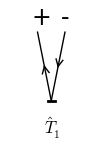
\includegraphics[width=46pt]{t1}
  \caption{}\label{fig:t1}
\endminipage\hfill
\minipage{.5\textwidth}
  \centering
  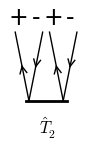
\includegraphics[width=44pt]{t2c}
  \caption{}\label{fig:t2}
\endminipage\hfill
\minipage{.5\textwidth}
  \centering
  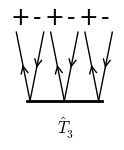
\includegraphics[width=60pt]{t3c}
  \caption{}\label{fig:t3}
\endminipage\hfill
\minipage{.5\textwidth}
  \centering
  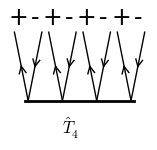
\includegraphics[width=80pt]{t4c}
  \caption{}\label{fig:t4}
\endminipage\hfill
\end{figure}

\begin{figure}
 \centering
  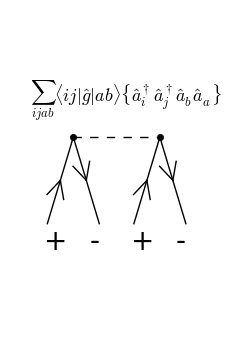
\includegraphics[width=120pt]{plusminus}
  \caption{Term in the normal ordered hamiltonian}\label{fig:plusminus}
\end{figure}

\subsection{Contractions of operators}

Analogous to Wicks's theorem, we need to find all possible ways to
contract the normal ordered Hamiltonian with strings of excitation
operators.  Our objective is thus to combine excitation operators,
possibly strings of excitation operators, with the various terms in
the normal ordered Hamiltonian, so they form topologically distinct
diagrams.

In Figs. \ref{fig:t1}, \ref{fig:t2}, \ref{fig:t3} and
\ref{fig:t4}, lines exiting the excitation operators are assigned a
number of plus and minus signs depending on the number of particle-
and hole lines in the operator. In the same way, we may assign plus or
minus signs to lines \emph{below} the interaction in the terms in the
normal ordered Hamiltonian. For strings of excitation operators, we
shall denote separations between the operators by a vertical line, so
that for example the product
\begin{equation}
\hat{T}_1 \hat{T}_2 \rightarrow + - \vert + - + - 
\label{eqn:exprod}
\end{equation}

Contractions will be represented diagrammatically as connecting
corresponding lines exiting the excitation operator and entering the
interaction vertex in the normal ordered Hamiltonian. The purpose of
the signs are to derive all topologically distinct connections between
these operators.

The plus and minus signs representing lines in the Hamiltonian term
must then \emph{all} connect to a corresponding sign in the string of
excitation operators, so that no lines entering or exiting below the
interaction is unconnected. At the same time, we seek only
combinations where at least one connection is made between the
Hamiltonian term and each of the excitation operators.

The practicalities of this procedure may be outlined in three steps.

First we must create any sequence containing the plus and minus signs
that occur in the Hamiltonian and the vertical bars from the string of
excitation operators. No vertical bars in this string of excitation operators means that we have only one operator, and that no such vertical bars should occur in the created sequence.

The next step is to consider all possible permutations of this
sequence. For each permutation we should first ensure that the diagram is \emph{linked} (see \ref{Chapter4}).

Contractions between the interaction and each of the excitation operators will be separated by
the vertical bars, so that unconnected operators may be identified by
either repeated vertical bars in the sequence as in
\begin{equation}
+ + \vert \vert - \vert -
\end{equation}
or by vertical bars at the start or end of the sequence as in

\begin{equation}
+ + \vert -\vert - \vert
\end{equation}

These connection patterns will correspond to unconnected diagrams and thus not contribute to the equations. 

Next, we need to ensure that the connection pattern is compatible to the operators, in the sense that the number
of connections of particle and holes ($+$ and $-$) to each excitation
operator must not exceed the corresponding plus and minus signs
present in the excitation operator.

As an example, we may consider the Hamiltonian term in Fig.
\ref{fig:plusminus} connecting to the string of operators in Eq.
(\ref{eqn:exprod}). These will together produce the sequence
\begin{equation}
\hat{H_{N,9}} \hat{T}_1 \hat{T}_2 \rightarrow  + - + - \vert 
\end{equation}

Now, in the order above this is obviously not a contributing term or
even a possible connection pattern, since there are no connections
between $\hat{H}_N$ and $\hat{T}_2$, and the number of connections to
$\hat{T}_1$ exceeds the possible number of connections to this
operator.

However, considering the possible permutations of this sequence will
enable us to identify three distinct connection patterns which are
\begin{equation}
  + -\vert  + - \hspace{1cm}  -\vert  + + -  \hspace{1cm}  + \vert  + - -
\end{equation}

From these three connection patterns we may draw three different
diagrams, shown in Fig. \ref{fig:ht1t2}. These diagrams will in turn be
translated back into algebraic expressions that we work into our code.
\begin{figure}
 \centering
  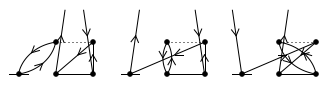
\includegraphics[width=320pt]{ht1t2}
  \caption{Diagrams produced by $\hat{H}_{N,9} \hat{T}_1 \hat{T}_2
    $. The diagrams are generated by our code and because of this the
    lines connect in a somewhat arbitrary fashion. Still, the diagrams
    are correct and non-ambiguous.}
\label{fig:ht1t2}
\end{figure}

A special case is when multiple occurrences of the same excitation
operators occur in the sequence. In this case the operators should be
treated as indistinguishable, so that only distinct connections occur.

For example we may consider the case of 

\begin{equation}
\hat{H_{N,9}} \hat{T}_2 \hat{T}_2 \rightarrow  + - + - \vert 
\end{equation}

The possible connection patterns from these operators are

\begin{equation}
  + -\vert  + - \hspace{1cm}  -\vert  + + -  \hspace{1cm}  + \vert  + - - \hspace{1cm}  ++ \vert  - -
\label{eqn:firstconnect}
\end{equation}

The last three terms could just as well be written

\begin{equation}
 + + -\vert  -  \hspace{1cm}  + - - \vert  + \hspace{1cm} - - \vert  + +
\end{equation}
but would not produce a diagram topologically distinct from the
connections in Eq. (\ref{eqn:firstconnect}), and is thereby excluded.


\subsection{Excitation level}

As may be seen from the diagrams in Fig. \ref{fig:ht1t2}, it is
fully possible for particles or holes in the excitation operator to
remain unconnected. In this case, we have three diagrams where all
have unconnected particle and hole lines. Such a diagram will produce
an excited Slater determinant, in this case creating a 1p1h (one
particle, one hole) state corresponding to the excitation level +1.

In other cases, we may have diagrams with no unconnected lines, corresponding to excitation level 0.

We will also have cases were particle and/or hole lines above the interaction cause excitations.

In general, we will find either zero or an even number of both particle- and hole lines unconnected in the diagram, and dividing the number of these by two will yield the excitation level.

The significance of the excitation level is that it quickly allows us to evaluate in which of the coupled cluster equations a diagram will contribute. Because of the orthonormality of the Slater determinants, only diagrams of excitation level 0 will contribute to the energy. Only diagrams of excitation level 2 will contribute to the t2-amplitude equation, and so on.

\subsection{Interpretation rules for diagrams}

Once all possible diagrams for a given sequence of operators are drawn, we will interpret them back into algebraic expressions that can be worked into code. The rules for interpreting diagrams are here just stated, pretty much as they appear in Shavitt and Bartlett's \emph{"Many Body Methods in Chemistry and Physics"} \cite[Chapter 9]{ShavittBartlett2009}.

\subsection{Label all lines}

Internal and external particle and hole lines are assigned labels. For consistency and readability one should use the conventional naming with letters \emph{"abcd..."} reserved for particles, and \emph{"ijkl..."} for holes. Since the diagrams represents sum over (internal) lines, it is preferable to reserve certain labels for summation indices and other for "static" indices. This will be helpful when writing the actual code.

\subsection{Identify the one-body operator}
Every one body vertex should be interpreted as the one body operator of the states exciting and entering the vertex, so that it produces an expression of the form $\hat{f}(p,q)$.

\subsection{Identify the two-body operator}
The two-body operator is identified as the two-body vertex with a dotted horizontal line, and the labels entering and/or leaving the vertex produce the following interaction:

\begin{equation}
\langle left out, right out \vert \vert left in, right in \rangle
\end{equation}

\subsection{Identify the amplitudes}
Each amplitude will occur as solid horizontal lines with particles and holes above it. Depending on the labeling, they are denoted algebraically as $\hat{t}^a_i$, $\hat{t}^{ab}_{ij}$, $\hat{t}^{abc}_{ijk}$ and $\hat{t}^{abcd}_{ijkl}$, for $\hat{T}_1$,$\hat{T}_2$,$\hat{T}_3$ and $\hat{T}_4$ respectively.

\subsection{Summation indices}
We then sum over all so-called internal indices that connects the amplitudes to the interaction. These are easily identified as the only connected lines in the diagram.

\subsection{Identify equivalent internal lines}
Equivalent lines are pairs of lines that connect at the same amplitude and interaction, in the same direction (particle-particle or hole-hole). For each such pair, we multiply the expression by a factor of $\frac{1}{2}$.

\subsection{Identify equivalent \emph{T}-vertices}
T-vertices are considered equivalent if they connect to the same interaction vertex in the same configurational pattern. For each such pair, multiply by a factor of $\frac{1}{2}$.

\subsection{The phase factor}
Count the number of hole lines and loops, and multiply the expression with a phase factor given by $(-)^{n_{holes}-n_{loops}}$. The number of holes is the number of lines pointing downwards, and a loop is easily identified as a pair of particle and hole lines connecting to the same two vertices.\footnote{Actually it is possible to draw diagrams in a manner that makes these loops hard to spot, but we shall not concern ourselves about this here.}

\subsection{External permutations}
A pair of external lines (unconnected lines) are considered equivalent if they connect to the same vertex. We must sum over all inequivalent external lines, and include a parity factor of $(-)^{\sigma(P)}$ where $\sigma(P)$ is the number of permutations.

\subsection{Cancel factors caused by external permutations}
For each pair of external lines connected to equivalent vertices, cancel one factor of $\frac{1}{2}$ caused by equivalent \emph{T}-vertices. 

\subsection{The correlation energy}
As may be seen from the energy equation (see Eq. (\ref{eqn:ccm1})), the diagrams that occur in this equation should have excitation level 0. When considering possible diagrams, this obviously means that the Hamiltonian term should not have any unconnected lines above the interaction, while all lines from the amplitudes should be connected to the interaction. In other words, we seek diagrams composed of only internal lines.

The only terms in the Hamiltonian that fulfill these criterions are the ones where all lines occur below the interaction, shown in Figs. \ref{fig:h1} and \ref{fig:h_9}. Considering the excitation level of these interactions, we find that they cause an excitation level of -1 for Fig. \ref{fig:h1} and -2 for Fig. \ref{fig:h_9}.

\begin{figure}[!h9h1]
\minipage{.5\textwidth}
  \centering
  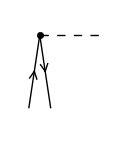
\includegraphics[width=46pt]{h1}
  \caption{}\label{fig:h1}
\endminipage\hfill
\minipage{.5\textwidth}
  \centering
  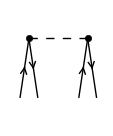
\includegraphics[width=44pt]{h_9}
  \caption{}\label{fig:h_9}
\endminipage\hfill
\end{figure}

It is then quite clear that only very few combinations are possible.  For example, no excitation beyond doubles will enter the energy expression, since they will excite the reference state beyond the +2 level. Only the single excitation operator $\hat{T}_1$ (see Fig. \ref{fig:t1}) will be able to produce an excitation level of +1, and thus connect with the one body operator in Fig. \ref{fig:h1}. 

We will find a total of three different diagrams that contribute to the energy, shown in Figs. \ref{fig:e1}, \ref{fig:e2} and \ref{fig:e3}.

\begin{figure}[!ccenergy]
\minipage{.3\textwidth}
  \centering
  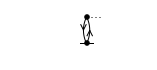
\includegraphics[width=100pt]{e1}
  \caption{}\label{fig:e1}
\endminipage\hfill
\minipage{.3\textwidth}
  \centering
  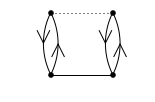
\includegraphics[width=80pt]{e2}
  \caption{}\label{fig:e2}
\endminipage\hfill
\minipage{.3\textwidth}
  \centering
  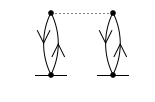
\includegraphics[width=80pt]{e3}
  \caption{}\label{fig:e3}
\endminipage\hfill
\end{figure}
 
To translate these diagrams into algebraic expressions, we apply the rules for diagram interpretation. We find 
\begin{equation}
\Delta e =  \sum_{ck} \langle k || c \rangle t_{k}^{c}+\frac{1}{4} \sum_{cdkl} \langle kl || cd \rangle t_{kl}^{cd}+\frac{1}{2} \sum_{ckdl} \langle kl || cd \rangle t_{k}^{c} t_{l}^{d}.
\label{eqn:c_energy}
\end{equation}

\section{Diagrams as code}

Although the diagrammatic rules greatly simplifies the process of
deriving the equations, there is still a high probability for errors
due to human inaccuracy. The CCSD $t1$ amplitude equations have for example 14
terms, making even the diagrammatic process quite tedious. This is
reflected even in authoritative works on the subjects such as Shavitt
and Bartlett's \emph{"Many Body Methods in Chemistry and Physics"}
\cite{ShavittBartlett2009}, where errors in the equations have been
found.\footnote{See as well Chapter 7 concerning the CCDT-1 validation.}

Hermann Kümmel noted in his "Biography of the Coupled Cluster Method"
\cite{Kummel}, that

\emph{"Because of the often large number of terms in all versions of the CCM it is rather hard work to obtain the explicit equations by hand. And after this is done one has to write a program to put them into the computer."}

Is it really necessary to derive equations by hand and thereafter
write code manually? Probably not, and for this reason it makes sense
to ensure consistency in the derivation process by use of
computers. If equations are derived by the computer, we may also task
the computer to actually generate the code needed for numerical
computation.

A number of symbolic frameworks that can handle such operations
exists such as \emph{Second Quantization} for SymPy (Python)
\cite{secondquant}, but these are based on the algebraic approach with
Wick's theorem. As a part of the work on this thesis, a python script
was developed aimed at deriving the CC equations at any level of truncation
using the diagrammatic approach.

In this section, we shall briefly discuss how to translate the
diagrammatic rules into code, and then proceed to derive the explicit
equations for various truncations by use of this code.

\subsection{Implementation}

We will need to define operators in terms of unconnected lines above
and below the interaction. It is natural to define a class for these
operators, and define functions such as contractions that takes
operator classes as parameters. A function for contractions of
operators should return all distinct diagrams for the operators.

An operator is sufficiently described by its number of hole- and
particle lines above and below the vertex. This is easily translated
into two arrays for each operator, with a binary representation of
particle or holes (for example 0 and 1).

To perform contractions of such operators, we will first need to set up the sequence of vertical bars and plus- and minus signs as previously described. This is basically just a new array, created by joining the array of particles and holes below the interaction vertex with a number of vertical bars equal to the number of excitation operators minus one.

The code then needs to seek through all possible permutations of this
sequence and identify the valid sequences. Such valid sequences may be
identified by connections between the Hamiltonian and all excitation
operators to its right, and by the number of connections occurring in
each excitation operator not exceeding the possible number of
connections.

Next we need to avoid over counting connection patterns due to
equivalent excitation operators, so we identify identical excitation
operators and keep only one of each such equivalent connection
pattern.

Finally we end up with a number of unique connection patterns that
gives us a non-ambiguous recipe for constructing the diagrams.

On top of this functionality we may want a framework for plotting the
diagrams or interpret them as algebraic expressions or code. IPython
Notebook \cite{ipython} provides an excellent environment for these
kinds of operations, so in the following sections we will explore
functionality in the script \emph{CCAlgebra} \cite{CCAlgebra}.\footnote{Note that parts of this script was developed by the author independently from this thesis, but by gradually including more functionality the author found that this code could easily be used as a tool directly in the work presented here.}

\subsection{CCAlgebra}

CCAlgebra is a python script that may be imported into any IPython
notebook. It has no dependencies outside those libraries that are
normally included in extended python distributions such as Entougth
Canopy \cite{Entought} or Continuum Analytics Anaconda
\cite{Anaconda}.

To start a session one just starts IPython Notebook and imports the
CCAlgebra.py file into the notebook.
It is then possible to define operators in the following manner

\begin{minipage}{\linewidth}
\makebox[\linewidth]{
  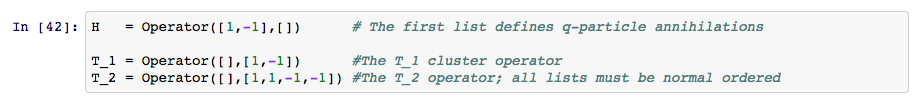
\includegraphics[keepaspectratio=true,scale=.5]{cca1}}  
\end{minipage}

Above we defined three operators; the Hamiltonian term from Fig.
\ref{fig:h1}, and the single and double excitation operators
$\hat{T}_1$ and $\hat{T}_2$. Each operator is fully described by two
lists; the first representing the pseudo particle annihilation
operators, while the second represents pseudo particle creation
operators.

To contract these operators we use a function that takes the
Hamiltonian operator and a list of excitation operators as parameters.

\begin{minipage}{\linewidth}
\makebox[\linewidth]{
  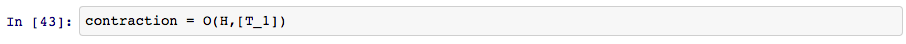
\includegraphics[keepaspectratio=true,scale=.5]{cca2}}  
\end{minipage}

This will return an object that contains all possible diagrams
generated from the contraction of these operators. The reason for that
excitation operators should be brace-enclosed in a list is that this
list contains all excitation operators to the right of the
Hamiltonian, consistent with the prior derivation from the Hausdorff
expansion.

Some simple information may be obtained from the resulting contraction, such as the excitation level and the number of resulting distinct diagrams

\begin{minipage}{\linewidth}
\makebox[\linewidth]{
  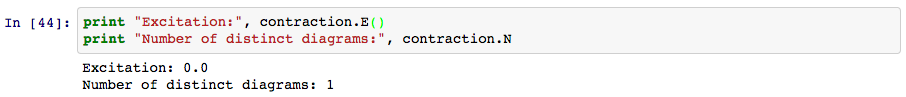
\includegraphics[keepaspectratio=true,scale=.5]{cca3}}  
\end{minipage}

The resulting diagrams are numbered from 0 and up, so as we only have one diagram resulting from this contraction we may display it as latex formatted text by the \emph{.latex()} method

\begin{minipage}{\linewidth}
\makebox[\linewidth]{
  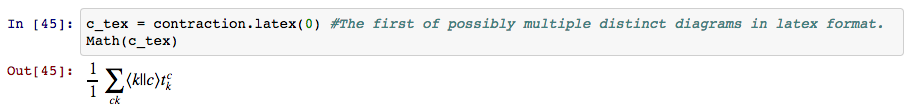
\includegraphics[keepaspectratio=true,scale=.5]{cca4}}  
\end{minipage}

We may also display it as a diagram by using the \emph{.diagram()} method.

\begin{minipage}{\linewidth}
\makebox[\linewidth]{
  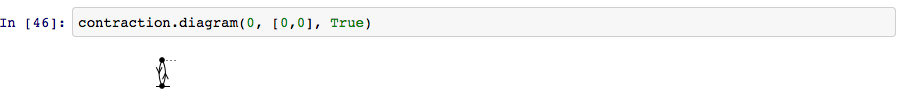
\includegraphics[keepaspectratio=true,scale=.5]{cca5}}  
\end{minipage}

The first parameter here specifies the number of the diagram
(beginning with 0), coordinates on the screen if we would like to
display multiple diagrams in the same frame, and finally an on/off
option for using built in formatting (turning of axis and scaling) or
letting the outside script adjust these parameters ("false").

With the computer's understanding of the diagram it is now very easy to translate it directly into code:

\begin{minipage}{\linewidth}
\makebox[\linewidth]{
  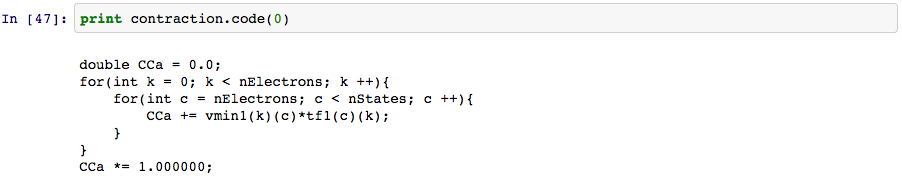
\includegraphics[keepaspectratio=true,scale=.5]{cca6}}  
\end{minipage}

In this case, the code is a naive C++ implementation (\emph{naive} in
the sense that it is the most direct translation of the diagram, using
for-loops where sums occur), but in principle it is possible to
generate any kind of code. Quite possibly also highly optimized code
if we supply the CCAlgebra script with some more information about the
system we want to calculate.

Terms in the CC equations may now be represented as code, diagrams or
mathematical expressions depending on how we prefer to view them, so it does make sense to
refer to these terms simply as "diagrams".

We may of course now easily derive more complex diagrams, simply by defining the operators we seek:

\begin{minipage}{\linewidth}
\makebox[\linewidth]{
  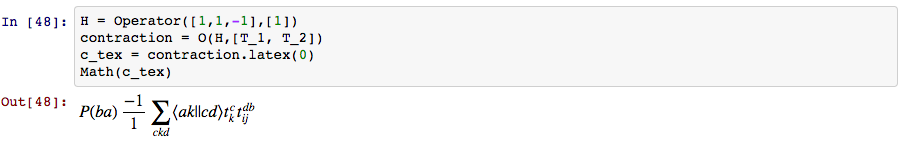
\includegraphics[keepaspectratio=true,scale=.5]{cca7}}  
\end{minipage}

Many physicists find diagrams helpful to quickly gain insight into the
nature of a given contribution, so we added functionality to quickly render diagrams on screen.

\begin{minipage}{\linewidth}
\makebox[\linewidth]{
  \includegraphics[keepaspectratio=true,scale=.5]{cca8}}  
\end{minipage}

In this case we used a two body term from the Hamiltonian, and we sum
over three internal lines. This results in a more computationally
intensive code with three nested for-loops:

\begin{minipage}{\linewidth}
\makebox[\linewidth]{
  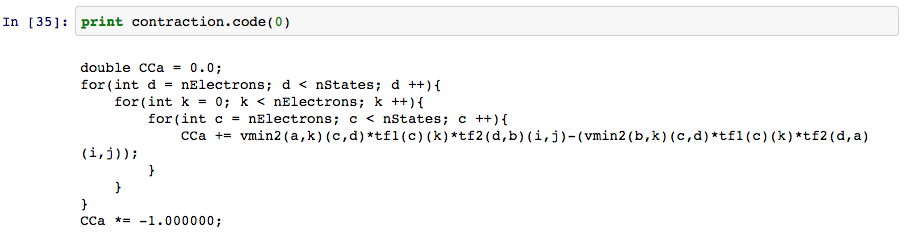
\includegraphics[keepaspectratio=true,scale=.5]{cca9}}  
\end{minipage}

In our equations the cluster operator occurs in a power series,
resulting in a multitude of products of excitation operators. To
handle this more easily and avoid the need to precalculate these, some
complementary functions to quickly evaluate such expanded power series
of the cluster operator is included:

\begin{minipage}{\linewidth}
\makebox[\linewidth]{
  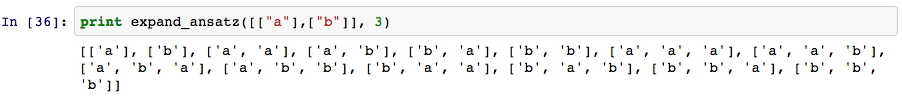
\includegraphics[keepaspectratio=true,scale=.5]{cca10}}  
\end{minipage}

It is also convenient to predefine some operators that occur often. A normal ordered Hamiltonian will come in handy:

\begin{minipage}{\linewidth}
\makebox[\linewidth]{
  \includegraphics[keepaspectratio=true,scale=.5]{cca11}}  
\end{minipage}

\subsection{Deriving amplitude equations using CCAlgebra}

Another convenient tool is a function that produces all possible
diagrams with a given excitation level from a normal ordered
Hamiltonian and the expanded exponential ansatz, in effect generating
the full energy- and amplitude equations. In the following example we
find all contributions to the t1 amplitude equation in the CCSD
truncation ($\hat{T} = \hat{T}_1 + \hat{T}_2$)

\begin{minipage}{\linewidth}
\makebox[\linewidth]{
  \includegraphics[keepaspectratio=true,scale=.5]{cca12}}  
\end{minipage}

The diagram are still a bit awkwardly formatted, but they are correct:

\begin{minipage}{\linewidth}
\makebox[\linewidth]{
  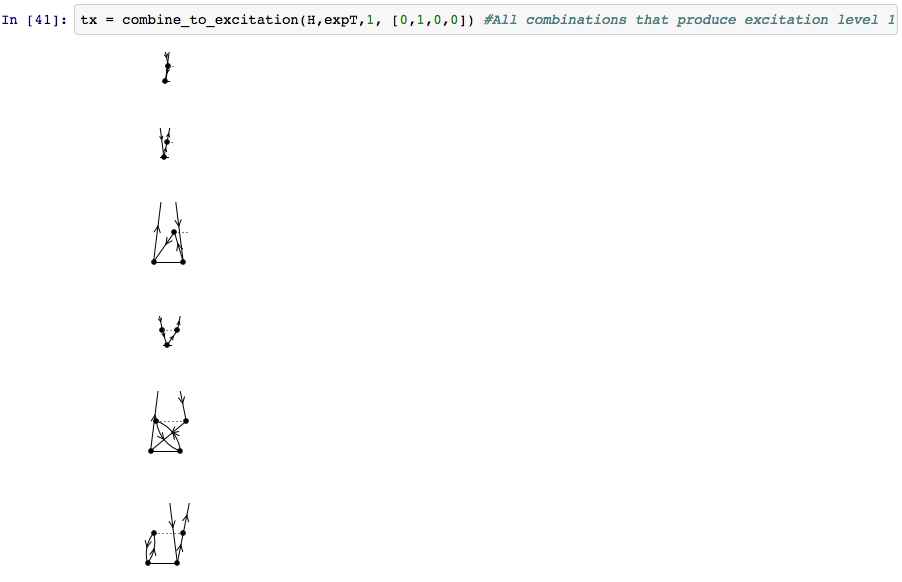
\includegraphics[keepaspectratio=true,scale=.5]{cca13}}  
\end{minipage}

\subsection{Deriving the energy using CCalgebra}

We have already noted how only a very few terms enter the energy
equations. Using CCAlgebra we may confirm that this is the indeed the
case

\begin{minipage}{\linewidth}
\makebox[\linewidth]{
  \includegraphics[keepaspectratio=true,scale=.5]{cca15}}  
\end{minipage}
By using CCAlgebra we may now go on to derive the explicit equations for the various CC methods. 

\subsection{Validation of CCAlgebra}

The developement of the CCAlgebra framework was mainly intended as an educational tool for better understanding of the CC equations and their derivation. As such, the code is written mainly as a proof of concept. 

Although the generated code from CCAlgebra is not optimized to such an extent that it will be usable for the system we explore in this thesis, it is fully capable to generate code that reproduce accurate results for well-known systems such as CCSD dissociation energies for the hydrogen molecule using a Gaussian basis set, as briefly described in the section on size consistency. The code generated by CC algebra was in exact agreement with the handwritten code in the CCSD case with only minor manual edits in the C++ code.

To a certain extent this validates the results obtained by the use of CCAlgebra, but it is still highly recommended to compare the equations and diagrams with the ones present in the literature before implementation.

\section{The CCD equations}

If we include only the double excitation operator in our cluster operator we get the CCD (Coupled Cluster Doubles) equations. This means we let 
\begin{equation}
\hat{T} = \hat{T}_2.
\end{equation}
We then perform the contractions with CCAlgebra. Since no single
excitations is included, we get an even simpler expression for the
energy than what we had earlier
\begin{equation}
\Delta e = \frac{1}{4} \sum_{cdkl} \langle kl || cd \rangle t_{kl}^{cd}.
\end{equation}

The only amplitude equation in this truncation is for $t2$:
\begin{multline}
0 =\langle ab \vert \vert ij \rangle + 
P(ij) \sum_{k} f_{kj} t_{ki}^{ab}+P(ab) \sum_{c} f_{bc} t_{ij}^{ac}+
\frac{1}{2} \sum_{cd} \langle ab \vert \vert cd \rangle t_{ij}^{cd} \\
+\frac{1}{2} \sum_{kl} \langle kl \vert \vert ij \rangle t_{kl}^{ab}-
P(ba)P(ij) \sum_{ck} \langle ak \vert \vert cj \rangle t_{ik}^{cb}- 
P(ij)\frac{1}{2} \sum_{cdkl} \langle kl \vert \vert cd \rangle t_{ik}^{cd} t_{jl}^{ab}\\
+\frac{1}{4} \sum_{cdkl} \langle kl \vert \vert cd \rangle t_{ij}^{cd} t_{kl}^{ab}-
 P(ab)\frac{1}{2} \sum_{ckld} \langle kl \vert \vert cd \rangle t_{kl}^{ca} t_{ij}^{db}+
P(ab)P(ij)\frac{1}{2} \sum_{ckdl} \langle kl \vert \vert cd \rangle t_{ik}^{ca} t_{jl}^{db}.
\end{multline}

There are a lot of different diagrams occurring in the CC
equations and it will make sense to classify them in ways that make
them more easily distinguishable. What is common to all diagrams is that
they contain only one Hamiltonian term contracted to possibly more
than one excitation operator. For this reason we may classify them
into orders of the various excitation operators occurring in them, and
in this simple case with only one excitation operator we may assign a
letter $L$ to diagrams \emph{linear} in $t2$ and the letter $Q$ to diagrams
\emph{quadratic} in $t2$. Since there are multiple diagrams
corresponding to each letter, we also assign a sub case letter in
their order of appearance.

The naming of each diagram is listed in table
\ref{tab:CCD_diagrams1}, but for now we just group together the terms
accordingly and define
\begin{multline}
L(t^{ab}_{ij}) \equiv 
\frac{1}{2} \sum_{cd} \langle ab \vert \vert cd \rangle t_{ij}^{cd} +
\frac{1}{2} \sum_{kl} \langle kl \vert \vert ij \rangle t_{kl}^{ab}-
P(ba)P(ij) \sum_{ck} \langle ak \vert \vert cj \rangle t_{ik}^{cb} .\\ 
\end{multline}
\begin{multline}
Q(t^{ab}_{ij}t^{ab}_{ij}) \equiv 
P(ij)\frac{1}{2} \sum_{cdkl} \langle kl \vert \vert cd \rangle t_{ik}^{cd} t_{jl}^{ab} 
+\frac{1}{4} \sum_{cdkl} \langle kl \vert \vert cd \rangle t_{ij}^{cd} t_{kl}^{ab} \\ - 
P(ab)\frac{1}{2} \sum_{ckld} \langle kl \vert \vert cd \rangle t_{kl}^{ca} t_{ij}^{db}+
P(ab)P(ij)\frac{1}{2} \sum_{ckdl} \langle kl \vert \vert cd \rangle t_{ik}^{ca} t_{jl}^{db},
\end{multline}
and write the CCD equation
\begin{equation}
0 =\langle ab \vert \vert ij \rangle + P(ij) \sum_{k} f_{kj} t_{ki}^{ab}+P(ab) \sum_{c} f_{bc} t_{ij}^{ac} + L(t^{ab}_{ij}) + Q(t^{ab}_{ij}t^{ab}_{ij}).
\end{equation}
It is not immediately clear how we are supposed to solve this
equation, but it is possible to rearrange the terms so that a
self-consistency criteria is found. This may be done by factoring out
the diagonal elements in the diagrams containing the one-body
operator, so that
\begin{equation}
P(ij) \sum_{k} f_{kj} t_{ki}^{ab} = \sum_{k \neq j} f_{kj} t_{ki}^{ab} + f_{jj} t_{ji}^{ab} - \sum_{k \neq i} f_{ki} t_{kj}^{ab}   - f_{ii} t_{ij}^{ab} =  -(f_{jj} + f_{ii}) t_{ij}^{ab} + \sum_{k \neq j} f_{kj} t_{ki}^{ab}  - \sum_{k \neq i} f_{ki} t_{kj}^{ab}  ,
\end{equation}
and
\begin{equation}
P(ab) \sum_{c} f_{ac} t_{ij}^{cb} = \sum_{c \neq a} f_{ac} t_{ij}^{cb} + f_{aa} t_{ij}^{ab} - \sum_{c \neq b} f_{bc} t_{ij}^{ca} -   f_{bb} t_{ij}^{ba} = (f_{aa} + f_{bb}) t_{ij}^{ab} +  \sum_{c \neq a} f_{ac} t_{ij}^{cb} - \sum_{c \neq b} f_{bc} t_{ij}^{ca}.
\end{equation}

In a canonical Hartree-Fock basis the one-body operator will only
contain diagonal elements, and since we will do all upcoming
calculations in such a basis we might as well ignore these non-diagonal sums. The full CCD amplitude equation then becomes
\begin{equation}
0 =\langle ab \vert \vert ij \rangle -(f_{jj} + f_{ii}) t_{ij}^{ab}+(f_{aa} + f_{bb}) t_{ij}^{ab}+L(t^{ab}_{ij}) + Q(t^{ab}_{ij}t^{ab}_{ij}).
\end{equation}
We may rewrite this expression to
\begin{equation}
 t_{ij}^{ab} =\frac{\langle ab \vert \vert ij \rangle+L(t^{ab}_{ij}) + Q(t^{ab}_{ij}t^{ab}_{ij})}{f_{jj} + f_{ii} - f_{aa} - f_{bb} }.
\end{equation}
With this expression we will be able to iteratively obtain self
consistence of the amplitudes. A reasonable guess for initial value
for the amplitudes is found by letting the $L$ and $Q$ term be zero,
so we have
\begin{equation}
 t_{ij}^{ab} =\frac{\langle ab \vert \vert ij \rangle}{f_{jj} + f_{ii} - f_{aa} - f_{bb} }.
\label{eqn:initialguess}
\end{equation}
These amplitudes actually correspond to the second order many-body perturbation energy, since
the evaluation of the energy expression for the CCD upon initialization yields
\begin{equation}
\Delta e^{(2)} =\frac{\langle ij \vert \vert ab \rangle \langle ab \vert \vert ij \rangle}{f_{jj} + f_{ii} - f_{aa} - f_{bb} }.
\label{eqn:initialenergy}
\end{equation}


\begin{table}[]
\centering
\caption{Diagrams CCD amplitude equation}
\label{tab:CCD_diagrams1}
\begin{tabular}{lllll}
Name & Factor & Permutation & Interpretation & Diagram \\
$$ & $-1$ & $P(ba)$ &$ \sum_{c} f_{a, c} t_{ij}^{cb}$  & 
\includegraphics[height=10mm]{CCD_0_3_0.png} \\  
$$ &  & $P(ij)$ &$ \sum_{k} f_{k, j} t_{ik}^{ab}$  & 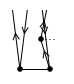
\includegraphics[height=10mm]{CCD_1_3_0.png} \\ 
$L_a$ & $\frac{1}{2}$ & &$ \sum_{cd} \langle ab \vert \vert cd \rangle t_{ij}^{cd}$  & 
\includegraphics[height=10mm]{CCD_4_3_0.png} \\  
$L_b$ & $\frac{1}{2}$ & &$ \sum_{kl} \langle kl \vert \vert ij \rangle t_{kl}^{ab}$  & 
\includegraphics[height=10mm]{CCD_5_3_0.png} \\ 
$L_c$ & $-1$ & $P(ba)P(ij)$ &$ \sum_{ck} \langle ak \vert \vert cj \rangle t_{ik}^{cb}$  & 
\includegraphics[height=10mm]{CCD_6_3_0.png} \\ 
$Q_a (D_{3a}) $ & $\frac{1}{4}$ & $$ &$ \sum_{cdkl} \langle kl \vert \vert cd \rangle t_{ij}^{cd} t_{kl}^{ab}$  & 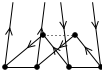
\includegraphics[height=10mm]{CCSD_t2_12_12_1.png} \\
$Q_b (D_{3b})  $ & $\frac{1}{2}$ & $P(ab)P(ij)$ &$ \sum_{ckdl} \langle kl \vert \vert cd \rangle t_{ik}^{ca} t_{jl}^{db}$  & 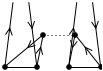
\includegraphics[height=10mm]{CCSD_t2_12_12_3.png} \\
$Q_c (D_{3c}) $ & $-\frac{1}{2}$ & $P(ab)$ &$ \sum_{ckld} \langle kl \vert \vert cd \rangle t_{kl}^{ca} t_{ij}^{db}$  & 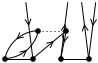
\includegraphics[height=10mm]{CCSD_t2_12_12_2.png} \\
$Q_d (D_{3d}) $ & $-\frac{1}{2}$ & $P(ij)$ &$ \sum_{cdkl} \langle kl \vert \vert cd \rangle t_{ik}^{cd} t_{jl}^{ab}$  & 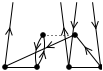
\includegraphics[height=10mm]{CCSD_t2_12_12_0.png} \\
\end{tabular}
\end{table}

\FloatBarrier


\section{The CCSD equations}
To improve upon the results from the CCD truncation the next step is to include single excitations from the $\hat{T}_1$ excitation operator. Although no such excitations occur on the system subject to this thesis, we review this contributions here for completeness. 

By inclusion of the single excitations, we have the cluster operator
\begin{equation}
\hat{T} = \hat{T}_1 + \hat{T}_2.
\end{equation}
The diagrams contributing to the amplitude equations for $t1$
and $t2$ are given in tables \ref{tab:CCSD_t1_correct} and
\ref{tab:CCSD_t2_correct1} \ref{tab:CCSD_t2_correct1}.

In the same way as for the $t2$ amplitude, we may factor out terms from
diagrams $S_{3a}$ and $S_{3b}$ to initialize the $t1$ amplitude, resulting in
\begin{equation}
t_i^a = \frac{f_{a,i}}{f(i,i) - f(a,a)}  .
\end{equation}
The next amplitude is found in the same manner as for the $t2$ amplitude
for the CCD approximation, and we iterate until some convergence
criteria is fulfilled.

%Sign inconsistencies: S5a, D5a,  D6a, D6b

%Errors: S6 (occurred triply, treated t_1 as distinguishable)

%Not interpreted properly (interaction) D4a, D4b (manually corrected)

%check later: D8b

\begin{table}[]
\centering
\caption{Contributions to the CCSD $\hat{T}_1$ amplitude equation}
\label{tab:CCSD_t1_correct}
\begin{tabular}{lllll}
Name & Factor & Permutation & Interpretation & Diagram\\
$S_{3a}$ &  & $$ &$ \sum_{c} f_{a, c} t_{i}^{c}$  & 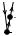
\includegraphics[height=10mm]{CCSD_t1_1_9_0.png} \\
$S_{3b}$ & $-1$ & $$ &$ \sum_{k} f_{k, i} t_{k}^{a}$  & 
\includegraphics[height=10mm]{CCSD_t1_0_9_0.png} \\
$S_{5a}$ &  & $$ &$ \sum_{ck} f_{k, c} t_{i}^{c} t_{k}^{a}$  & 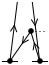
\includegraphics[height=10mm]{CCSD_t1_3_5_0.png} \\
$S_{2a}$ &  & $$ &$ \sum_{ck} f_{k, c} t_{ik}^{ca}$  & 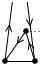
\includegraphics[height=10mm]{CCSD_t1_3_13_0.png} \\
$S_{3c}$ & $-1$ & $$ &$ \sum_{ck} \langle ak \vert \vert ci \rangle t_{k}^{c}$  & 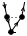
\includegraphics[height=10mm]{CCSD_t1_6_9_0.png} \\
$S_{5b}$ &  & $$ &$ \sum_{ckd} \langle ak \vert \vert cd \rangle t_{k}^{c} t_{i}^{d}$  & 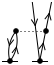
\includegraphics[height=10mm]{CCSD_t1_10_5_0.png} \\
$S_{2b}$ & $\frac{1}{2}$ & $$ &$ \sum_{cdk} \langle ak \vert \vert cd \rangle t_{ik}^{cd}$  & 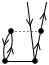
\includegraphics[height=10mm]{CCSD_t1_10_13_0.png} \\
$S_{5c}$ & $-1$ & $$ &$ \sum_{ckl} \langle kl \vert \vert ci \rangle t_{k}^{c} t_{l}^{a}$  & 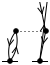
\includegraphics[height=10mm]{CCSD_t1_8_5_0.png} \\
$S_{2c}$ & $-\frac{1}{2}$ & $$ &$ \sum_{ckl} \langle kl \vert \vert ci \rangle t_{kl}^{ca}$  & 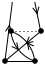
\includegraphics[height=10mm]{CCSD_t1_8_13_0.png} \\
$S_6$ &  & $$ &$ \sum_{ckdl} \langle kl \vert \vert cd \rangle t_{i}^{c} t_{k}^{a} t_{l}^{d}$  & 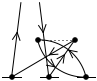
\includegraphics[height=10mm]{CCSD_t1_12_2_1.png} \\
$S_{4c}$ &  & $$ &$ \sum_{ckdl} \langle kl \vert \vert cd \rangle t_{k}^{c} t_{il}^{da}$  & 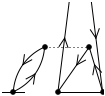
\includegraphics[height=10mm]{CCSD_t1_12_8_0.png} \\
$S_{4a}$ & $\frac{1}{2}$ & $$ &$ \sum_{cdkl} \langle kl \vert \vert cd \rangle t_{i}^{c} t_{kl}^{da}$  & 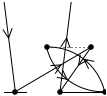
\includegraphics[height=10mm]{CCSD_t1_12_8_2.png} \\
$S_{4b}$ & $\frac{1}{2}$ & $$ &$ \sum_{kcdl} \langle kl \vert \vert cd \rangle t_{k}^{a} t_{il}^{cd}$  & 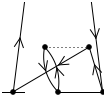
\includegraphics[height=10mm]{CCSD_t1_12_8_1.png} \\
\end{tabular}
\end{table}

\begin{table}[]
\centering
\caption{Contributions to the CCSD $\hat{T}_2$ amplitude equation (1)}
\label{tab:CCSD_t2_correct1}
\begin{tabular}{lllll}
Name & Factor & Permutation & Interpretation & Diagram\\
$$ & $-1$ & $P(ba)$ &$ \sum_{c} f_{a, c} t_{ij}^{cb}$  & 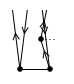
\includegraphics[height=10mm]{CCD_1_3_0.png} \\  
$$ &  & $P(ij)$ &$ \sum_{k} f_{k, j} t_{ik}^{ab}$  & 
\includegraphics[height=10mm]{CCD_0_3_0.png} \\ 
$L_a$ & $\frac{1}{2}$ & &$ \sum_{cd} \langle ab \vert \vert cd \rangle t_{ij}^{cd}$  & \includegraphics[height=10mm]{CCD_5_3_0.png} \\  
$L_b$ & $\frac{1}{2}$ & &$ \sum_{kl} \langle kl \vert \vert ij \rangle t_{kl}^{ab}$  & \includegraphics[height=10mm]{CCD_4_3_0.png} \\ 
$L_c$ & $-1$ & $P(ba)P(ij)$ &$ \sum_{ck} \langle ak \vert \vert cj \rangle t_{ik}^{cb}$  & \includegraphics[height=10mm]{CCD_6_3_0.png} \\ 
$D_{3a} $ & $\frac{1}{4}$ & $$ &$ \sum_{cdkl} \langle kl \vert \vert cd \rangle t_{ij}^{cd} t_{kl}^{ab}$  & \includegraphics[height=10mm]{CCSD_t2_12_12_1.png} \\
$D_{3b}  $ & $\frac{1}{2}$ & $P(ab)P(ij)$ &$ \sum_{ckdl} \langle kl \vert \vert cd \rangle t_{ik}^{ca} t_{jl}^{db}$  & \includegraphics[height=10mm]{CCSD_t2_12_12_3.png} \\
$D_{3c} $ & $-\frac{1}{2}$ & $P(ab)$ &$ \sum_{ckld} \langle kl \vert \vert cd \rangle t_{kl}^{ca} t_{ij}^{db}$  & \includegraphics[height=10mm]{CCSD_t2_12_12_0.png} \\
$D_{3d} $ & $-\frac{1}{2}$ & $P(ij)$ &$ \sum_{cdkl} \langle kl \vert \vert cd \rangle t_{ik}^{cd} t_{jl}^{ab}$  & \includegraphics[height=10mm]{CCSD_t2_12_12_2.png} \\
$D_{5a}$ & $-1$ & $P(ij)$ &$ \sum_{ck} f_{k, c} t_{i}^{c} t_{jk}^{ab}$  & \includegraphics[height=10mm]{CCSD_t2_3_8_1.png} \\
$D_{5b}$ & $-1$ & $P(ab)$ &$ \sum_{kc} f_{k, c} t_{k}^{a} t_{ij}^{cb}$  & \includegraphics[height=10mm]{CCSD_t2_3_8_0.png} \\
$D_{6a}$ & $-\frac{1}{2}$ & $P(ij)$ &$ \sum_{cd} \langle ab \vert \vert cd \rangle t_{i}^{c} t_{j}^{d}$  & \includegraphics[height=10mm]{CCSD_t2_5_5_0.png} \\
$D_{6b}$ & $-\frac{1}{2}$ & $P(ab)$ &$ \sum_{kl} \langle kl \vert \vert ij \rangle t_{k}^{a} t_{l}^{b}$  & \includegraphics[height=10mm]{CCSD_t2_4_5_0.png} \\
$D_{6c}$ & $-1$ & $P(ij)P(ba)$ &$ \sum_{ck} \langle ak \vert \vert cj \rangle t_{i}^{c} t_{k}^{b}$  & \includegraphics[height=10mm]{CCSD_t2_6_5_0.png} \\
$D_{4a}$ &  & $P(ij)$ &$ \sum_{c}  \langle ab \vert \vert cj \rangle t_{i}^{c}$  & \includegraphics[height=10mm]{CCSD_t2_9_9_0.png} \\
$D_{8a}$ & $\frac{1}{2}$ & $P(ij)P(ba)$ &$ \sum_{cdk} \langle ak \vert \vert cd \rangle t_{i}^{c} t_{j}^{d} t_{k}^{b}$  & \includegraphics[height=10mm]{CCSD_t2_10_2_0.png} \\
$D_{8b}$ & $\frac{1}{2}$ & $P(ij)P(ba)$ &$ \sum_{cdk} \langle ak \vert \vert cd \rangle t_{i}^{c} t_{j}^{d} t_{k}^{b}$  & \includegraphics[height=10mm]{CCSD_t2_8_2_0.png} \\
$D_{5g}$ & $-1$ & $P(ba)$ &$ \sum_{ckd} \langle ak \vert \vert cd \rangle t_{k}^{c} t_{ij}^{db}$  & \includegraphics[height=10mm]{CCSD_t2_10_8_0.png} \\
$D_{5c}$ &  & $P(ij)P(ba)$ &$ \sum_{cdk} \langle ak \vert \vert cd \rangle t_{i}^{c} t_{jk}^{db}$  & \includegraphics[height=10mm]{CCSD_t2_10_8_2.png} \\
$D_{5e}$ & $-\frac{1}{2}$ & $P(ab)$ &$ \sum_{kcd} \langle kb \vert \vert cd \rangle t_{k}^{a} t_{ij}^{cd}$  & \includegraphics[height=10mm]{CCSD_t2_10_8_1.png} \\
$D_{4b}$ & $-1$ & $P(ab)$ &$ \sum_{k} \langle kb \vert \vert ij \rangle t_{k}^{a}$  & \includegraphics[height=10mm]{CCSD_t2_7_9_0.png} \\
\end{tabular}
\end{table}


\begin{table}[]
\centering
\caption{Contributions to the CCSD $\hat{T}_2$ amplitude equation (2)}
\label{tab:CCSD_t2_correct2}
\begin{tabular}{lllll}
Name & Factor & Permutation & Interpretation & Diagram\\
$D_{8b}$ & $-\frac{1}{2}$ & $P(ij)P(ab)$ &$ \sum_{ckl} \langle kl \vert \vert cj \rangle t_{i}^{c} t_{k}^{a} t_{l}^{b}$  & \includegraphics[height=10mm]{CCSD_t2_10_2_0.png} \\
$D_{5h}$ &  & $P(ji)$ &$ \sum_{ckl} \langle kl \vert \vert ci \rangle t_{k}^{c} t_{jl}^{ab}$  & \includegraphics[height=10mm]{CCSD_t2_8_8_0.png} \\
$D_{5f}$ & $\frac{1}{2}$ & $P(ij)$ &$ \sum_{ckl} \langle kl \vert \vert cj \rangle t_{i}^{c} t_{kl}^{ab}$  & \includegraphics[height=10mm]{CCSD_t2_8_8_2.png} \\
$D_{5d}$ & $-1$ & $P(ab)P(ji)$ &$ \sum_{kcl} \langle kl \vert \vert ic \rangle t_{k}^{a} t_{jl}^{cb}$  & \includegraphics[height=10mm]{CCSD_t2_8_8_1.png} \\
$D_9$ & $\frac{1}{4}$ & $P(ij)P(ab)$ &$ \sum_{cdkl} \langle kl \vert \vert cd \rangle t_{i}^{c} t_{j}^{d} t_{k}^{a} t_{l}^{b}$  & \includegraphics[height=10mm]{CCSD_t2_12_0_0.png} \\
$D_{7d}$ & $-1$ & $P(ij)$ &$ \sum_{ckdl} \langle kl \vert \vert cd \rangle t_{k}^{c} t_{i}^{d} t_{jl}^{ab}$  & \includegraphics[height=10mm]{CCSD_t2_12_4_1.png} \\
$D_{7e}$ & $-1$ & $P(ab)$ &$ \sum_{ckld} \langle kl \vert \vert cd \rangle t_{k}^{c} t_{l}^{a} t_{ij}^{db}$  & \includegraphics[height=10mm]{CCSD_t2_12_4_0.png} \\
$D_{7a}$ & $-\frac{1}{4}$ & $P(ij)$ &$ \sum_{cdkl} \langle kl \vert \vert cd \rangle t_{i}^{c} t_{j}^{d} t_{kl}^{ab}$  & \includegraphics[height=10mm]{CCSD_t2_12_4_4.png} \\
$D_{7c}$ &  & $P(ij)P(ab)$ &$ \sum_{ckdl} \langle kl \vert \vert cd \rangle t_{i}^{c} t_{k}^{a} t_{jl}^{db}$  & \includegraphics[height=10mm]{CCSD_t2_12_4_3.png} \\
$D_{7b} $ & $-\frac{1}{4}$ & $P(ab)$ &$ \sum_{klcd} \langle kl \vert \vert cd \rangle t_{k}^{a} t_{l}^{b} t_{ij}^{cd}$  & \includegraphics[height=10mm]{CCSD_t2_12_4_2.png} \\
\end{tabular}
\end{table}

\FloatBarrier

\section{The CCSDT equations}

In this section we present the full CCSDT equations as they are
generated by CCAlgebra for completeness. A thorough (and authorative)
derivation and treatment of these equations may be found in
\cite{ShavittBartlett2009}. It should be noted that inconsistencies
were found between these equations and the ones derived in
\cite{ShavittBartlett2009} concerning the signs in diagrams $T_{1a}$,
$T_{1b}$, and that the signs as they appear in table
\ref{tab:CCSDT_diagrams3_correct} produced results more in agreement
with expectations. While the signs in \cite{ShavittBartlett2009}
produced CCD(T) energies above the CCD energy, the ones from CCAlgebra
produced energies lower than the CCD results (for the HEG 3D system),
as one would expect for our system.

For the CCSDT equations, we have the cluster operator

\begin{equation}
\hat{T} = \hat{T}_1 + \hat{T}_2 + \hat{T}_3.
\end{equation}

In table \ref{tab:CCSDT_t1}, all contributions to the CCSDT t1 equation are listed, and we find only one extra diagram compared to the CCSD truncation ($S_7$). The solution procedure for this equation will be the same as for the CCSD and t1 amplitudes.

In the CCSDT $t2$ amplitude, we find six additional diagrams when
comparing to the CCSD $t2$ amplitudes. The additional diagrams are
listed in table \ref{tab:CCSDT_t2}. The solution procedure for this
equation shall also be the same as for the CCSD and CCD $t2$ amplitudes,
by factoring out terms and using a self consistency procedure.

All contributions to the $t3$ amplitudes are listed in tables
\ref{tab:CCSDT_diagrams3_correct1} -
\ref{tab:CCSDT_diagrams3_correct2}. Following a similar factorization
procedure as for the previous equations, we may factor out terms from
diagrams $T_{2a}$ and $T_{2b}$ so we find

\begin{equation}
\epsilon^{abc}_{ijk} t^{abc}_{ijk} = T_{1a} + T_{1b} + T_{2c} + ... + T_{10a},
\label{eqn:t3_factor}
\end{equation}
where we have defined
\begin{equation}
\epsilon^{abc}_{ijk} = f(i,i) + f(j,j) + f(k,k) - f(a,a) - f(b,b) - f(c,c).
\label{eqn:t3_factor}
\end{equation}

\subsection{Computational cost}

The computational cost of the full CCSDT equation scales as $n_h^3
n_p^5$ per iteration, where $n_p$ is the number of particle states and
$n_h$ is the number of hole states \cite[p.316]{ShavittBartlett2009}.
This, as well as the fact that such amplitudes actually have to be
stored using $n_h^3 n_p^3$ preferably double precision floats, makes
implementation of the full CCSDT a formidable challenge.
 

\begin{table}[]
\centering
\caption{Contributions to the CCSDT $\hat{T}_1$ amplitude equation}
\label{tab:CCSDT_t1}
\begin{tabular}{lllll}
$S_{3a}$ &  & $$ &$ \sum_{c} f_{a, c} t_{i}^{c}$  & \includegraphics[height=10mm]{CCSD_t1_1_9_0.png} \\
$S_{3b}$ & $-1$ & $$ &$ \sum_{k} f_{k, i} t_{k}^{a}$  & \includegraphics[height=10mm]{CCSD_t1_0_9_0.png} \\
$S_{5a}$ &  & $$ &$ \sum_{ck} f_{k, c} t_{i}^{c} t_{k}^{a}$  & \includegraphics[height=10mm]{CCSD_t1_3_5_0.png} \\
$S_{2a}$ &  & $$ &$ \sum_{ck} f_{k, c} t_{ik}^{ca}$  & \includegraphics[height=10mm]{CCSD_t1_3_13_0.png} \\
$S_{3c}$ & $-1$ & $$ &$ \sum_{ck} \langle ak \vert \vert ci \rangle t_{k}^{c}$  & \includegraphics[height=10mm]{CCSD_t1_6_9_0.png} \\
$S_{5b}$ &  & $$ &$ \sum_{ckd} \langle ak \vert \vert cd \rangle t_{k}^{c} t_{i}^{d}$  & \includegraphics[height=10mm]{CCSD_t1_10_5_0.png} \\
$S_{2b}$ & $\frac{1}{2}$ & $$ &$ \sum_{cdk} \langle ak \vert \vert cd \rangle t_{ik}^{cd}$  & \includegraphics[height=10mm]{CCSD_t1_10_13_0.png} \\
$S_{5c}$ & $-1$ & $$ &$ \sum_{ckl} \langle kl \vert \vert ci \rangle t_{k}^{c} t_{l}^{a}$  & \includegraphics[height=10mm]{CCSD_t1_8_5_0.png} \\
$S_{2c}$ & $-\frac{1}{2}$ & $$ &$ \sum_{ckl} \langle kl \vert \vert ci \rangle t_{kl}^{ca}$  & \includegraphics[height=10mm]{CCSD_t1_8_13_0.png} \\
$S_6$ &  & $$ &$ \sum_{ckdl} \langle kl \vert \vert cd \rangle t_{i}^{c} t_{k}^{a} t_{l}^{d}$  & \includegraphics[height=10mm]{CCSD_t1_12_2_1.png} \\
$S_{4c}$ &  & $$ &$ \sum_{ckdl} \langle kl \vert \vert cd \rangle t_{k}^{c} t_{il}^{da}$  & \includegraphics[height=10mm]{CCSD_t1_12_8_0.png} \\
$S_{4a}$ & $\frac{1}{2}$ & $$ &$ \sum_{cdkl} \langle kl \vert \vert cd \rangle t_{i}^{c} t_{kl}^{da}$  & \includegraphics[height=10mm]{CCSD_t1_12_8_2.png} \\
$S_{4b}$ & $\frac{1}{2}$ & $$ &$ \sum_{kcdl} \langle kl \vert \vert cd \rangle t_{k}^{a} t_{il}^{cd}$  & \includegraphics[height=10mm]{CCSD_t1_12_8_1.png} \\
$S_7$ & $\frac{1}{4}$ & $$ &$ \sum_{cdkl} \langle kl \vert \vert cd \rangle t_{ikl}^{cda}$  & \includegraphics[height=10mm]{CCSDT_t1_12_33_0.png} \\
\end{tabular}
\end{table}


\begin{table}[]
\centering
\caption{Additional diagrams in the CCSDT $\hat{T}_2$ amplitude equation (1)}
\label{tab:CCSDT_t2}
\begin{tabular}{lllll}
Name & Factor & Permutation & Interpretation & Diagram\\
$D_{10a}$ &  & $$ &$ \sum_{ck} f_{k, c} t_{ijk}^{cab}$  & \includegraphics[height=10mm]{CCSD_t2_3_33_0.png} \\
$D_{10b}$ & $-\frac{1}{2}$ & $P(ba)$ &$ \sum_{cdk} \langle ak \vert \vert cd \rangle t_{ijk}^{cdb}$  & \includegraphics[height=10mm]{CCSD_t2_10_33_0.png} \\
$D_{10c}$ & $\frac{1}{2}$ & $P(ij)$ &$ \sum_{ckl} \langle kl \vert \vert cj \rangle t_{ikl}^{cab}$  & \includegraphics[height=10mm]{CCSD_t2_8_33_0.png} \\
$D_{11a}$ &  & $$ &$ \sum_{ckdl} \langle kl \vert \vert cd \rangle t_{k}^{c} t_{ijl}^{dab}$  & \includegraphics[height=10mm]{CCSD_t2_12_18_0.png} \\
$D_{11c}$ & $-\frac{1}{2}$ & $P(ij)$ &$ \sum_{cdkl} \langle kl \vert \vert cd \rangle t_{i}^{c} t_{jkl}^{dab}$  & \includegraphics[height=10mm]{CCSD_t2_12_18_2.png} \\
$D_{11b}$ & $-\frac{1}{2}$ & $P(ab)$ &$ \sum_{kcdl} \langle kl \vert \vert cd \rangle t_{k}^{a} t_{ijl}^{cdb}$  & \includegraphics[height=10mm]{CCSD_t2_12_18_1.png} \\
\end{tabular}
\end{table}


\begin{table}[]
\centering
\caption{Contributions to the CCSDT $\hat{T}_3$ amplitude equation (1)}
\label{tab:CCSDT_diagrams3_correct1}
\begin{tabular}{lllll}
Name & Factor & Permutation & Interpretation & Diagram\\
$T_{1a}$ & $-1$ & $P(ba)P(bz)P(iw)P(jw)$ &$ \sum_{c} \langle ab \vert \vert ck \rangle t_{ij}^{cb}$  & \includegraphics[height=10mm]{CC9_29_0.png} \\
$T_{1b}$ &  & $P(az)P(bz)P(ij)P(iw)$ &$ \sum_{k} \langle kz \vert \vert j \rangle t_{ik}^{ab}$  & \includegraphics[height=10mm]{CC7_29_0.png} \\
$T_{2a}$ &  & $P(ba)P(za)$ &$ \sum_{c} f_{a, c} t_{ijw}^{cbz}$  & \includegraphics[height=10mm]{CC1_33_0.png} \\
$T_{2b}$ & $-1$ & $P(iw)P(jw)$ &$ \sum_{k} f_{k, w} t_{ijk}^{abz}$  & \includegraphics[height=10mm]{CC0_33_0.png} \\
$T_{6a}$ &  & $P(ij)P(iw)$ &$ \sum_{ck} f_{k, c} t_{i}^{c} t_{jwk}^{abz}$  & \includegraphics[height=10mm]{CC3_18_1.png} \\
$T_{6b}$ &  & $P(ab)P(az)$ &$ \sum_{kc} f_{k, c} t_{k}^{a} t_{ijw}^{cbz}$  & \includegraphics[height=10mm]{CC3_18_0.png} \\
$T_{2c}$ & $\frac{1}{2}$ & $P(za)P(zb)$ &$ \sum_{cd} \langle ab \vert \vert cd \rangle t_{ijw}^{cdz}$  & \includegraphics[height=10mm]{CC5_33_0.png} \\
$T_{2d}$ & $\frac{1}{2}$ & $P(iw)P(ij)$ &$ \sum_{kl} \langle kl \vert \vert jw \rangle t_{ikl}^{abz}$  & \includegraphics[height=10mm]{CC4_33_0.png} \\
$T_{2e}$ & $-1$ & $P(ba)P(za)P(iw)P(jw)$ &$ \sum_{ck} \langle ak \vert \vert cw \rangle t_{ijk}^{cbz}$  & \includegraphics[height=10mm]{CC6_33_0.png} \\
$T_{3a}$ &  & $P(ab)P(az)P(iw)P(jw)$ &$ \sum_{ck} f_{k, c} t_{ij}^{ca} t_{wk}^{bz}$  & \includegraphics[height=10mm]{CC3_25_0.png} \\
$T_{3d}$ & $\frac{1}{2}$ & $P(iw)P(jw)P(ba)P(za)$ &$ \sum_{cdk} \langle ak \vert \vert cd \rangle t_{ij}^{cd} t_{wk}^{bz}$  & \includegraphics[height=10mm]{CC10_25_1.png} \\
$T_{3b}$ & $-1$ & $P(bz)P(ba)P(ij)P(iw)P(za)$ &$ \sum_{ckd} \langle ak \vert \vert cd \rangle t_{ik}^{cb} t_{jw}^{dz}$  & \includegraphics[height=10mm]{CC8_25_1.png} \\
$T_{3c}$ &  & $P(ab)P(az)P(iw)P(ij)P(wj)$ &$ \sum_{ckl} \langle kl \vert \vert cj \rangle t_{ik}^{ca} t_{wl}^{bz}$  & \includegraphics[height=10mm]{CC10_25_0.png} \\
$T_{3e}$ & $-\frac{1}{2}$ & $P(ab)P(az)P(iw)P(jw)$ &$ \sum_{ckl} \langle kl \vert \vert cw \rangle t_{ij}^{ca} t_{kl}^{bz}$  & \includegraphics[height=10mm]{CC8_25_0.png} \\
$T_{4a}$ &  & $P(ij)P(iw)P(za)P(zb)$ &$ \sum_{cd} \langle ab \vert \vert cd \rangle t_{i}^{c} t_{jw}^{dz}$  & \includegraphics[height=10mm]{CC5_15_0.png} \\
$T_{4b}$ &  & $P(ab)P(az)P(ji)P(jw)$ &$ \sum_{kl} \langle kl \vert \vert iw \rangle t_{k}^{a} t_{jl}^{bz}$  & \includegraphics[height=10mm]{CC4_15_0.png} \\
$T_{4c}$ &  & $P(ij)P(iw)P(ba)P(za)P(jw)$ &$ \sum_{ck} \langle ak \vert \vert cw \rangle t_{i}^{c} t_{jk}^{bz}$  & \includegraphics[height=10mm]{CC6_15_1.png} \\
$T_{4d}$ &  & $P(az)P(ab)P(zb)P(ji)P(wi)$ &$ \sum_{kc} \langle kb \vert \vert ic \rangle t_{k}^{a} t_{jw}^{cz}$  & \includegraphics[height=10mm]{CC6_15_0.png} \\
\end{tabular}
\end{table}

\begin{table}[]
\centering
\caption{Contributions to the CCSDT $\hat{T}_3$ amplitude equation (2)}
\label{tab:CCSDT_diagrams3_correct2}
\begin{tabular}{lllll}
$T_{6e}$ &  & $P(ba)P(za)$ &$ \sum_{ckd} \langle ak \vert \vert cd \rangle t_{k}^{c} t_{ijw}^{dbz}$  & \includegraphics[height=10mm]{CC10_18_0.png} \\
$T_{6c}$ &  & $P(ij)P(iw)P(ba)P(za)$ &$ \sum_{cdk} \langle ak \vert \vert cd \rangle t_{i}^{c} t_{jwk}^{dbz}$  & \includegraphics[height=10mm]{CC10_18_2.png} \\
$T_{6g}$ & $-\frac{1}{2}$ & $P(az)P(ab)P(zb)$ &$ \sum_{kcd} \langle kb \vert \vert cd \rangle t_{k}^{a} t_{ijw}^{cdz}$  & \includegraphics[height=10mm]{CC10_18_1.png} \\
$T_{6f}$ & $-1$ & $P(ji)P(wi)$ &$ \sum_{ckl} \langle kl \vert \vert ci \rangle t_{k}^{c} t_{jwl}^{abz}$  & \includegraphics[height=10mm]{CC8_18_0.png} \\
$T_{6h}$ & $\frac{1}{2}$ & $P(ij)P(iw)P(jw)$ &$ \sum_{ckl} \langle kl \vert \vert cw \rangle t_{i}^{c} t_{jkl}^{abz}$  & \includegraphics[height=10mm]{CC8_18_2.png} \\
$T_{6d}$ & $-1$ & $P(ab)P(az)P(ji)P(wi)$ &$ \sum_{kcl} \langle kl \vert \vert ic \rangle t_{k}^{a} t_{jwl}^{cbz}$  & \includegraphics[height=10mm]{CC8_18_1.png} \\
$T_{5b}$ & $\frac{1}{2}$ & $P(ij)P(iw)$ &$ \sum_{cdkl} \langle kl \vert \vert cd \rangle t_{ik}^{cd} t_{jwl}^{abz}$  & \includegraphics[height=10mm]{CC12_28_2.png} \\
$T_{5f}$ & $\frac{1}{4}$ & $P(iw)P(jw)$ &$ \sum_{cdkl} \langle kl \vert \vert cd \rangle t_{ij}^{cd} t_{wkl}^{abz}$  & \includegraphics[height=10mm]{CC12_28_5.png} \\
$T_{5c}$ & $\frac{1}{2}$ & $P(ab)P(az)$ &$ \sum_{ckld} \langle kl \vert \vert cd \rangle t_{kl}^{ca} t_{ijw}^{dbz}$  & \includegraphics[height=10mm]{CC12_28_0.png} \\
$T_{5a}$ &  & $P(ab)P(az)P(ij)P(iw)$ &$ \sum_{ckdl} \langle kl \vert \vert cd \rangle t_{ik}^{ca} t_{jwl}^{dbz}$  & \includegraphics[height=10mm]{CC12_28_3.png} \\
$T_{5d}$ & $\frac{1}{2}$ & $P(ab)P(az)P(iw)P(jw)$ &$ \sum_{cdkl} \langle kl \vert \vert cd \rangle t_{ij}^{ca} t_{wkl}^{dbz}$  & \includegraphics[height=10mm]{CC12_28_4.png} \\
$T_{5g}$ & $\frac{1}{4}$ & $P(az)P(bz)$ &$ \sum_{klcd} \langle kl \vert \vert cd \rangle t_{kl}^{ab} t_{ijw}^{cdz}$  & \includegraphics[height=10mm]{CC12_28_6.png} \\
$T_{5e}$ & $\frac{1}{2}$ & $P(az)P(bz)P(ij)P(iw)$ &$ \sum_{kcdl} \langle kl \vert \vert cd \rangle t_{ik}^{ab} t_{jwl}^{cdz}$  & \includegraphics[height=10mm]{CC12_28_1.png} \\
$T_{7c}$ & $-\frac{1}{2}$ & $P(ij)P(iw)P(jw)P(ba)P(za)$ &$ \sum_{cdk} \langle ak \vert \vert cd \rangle t_{i}^{c} t_{j}^{d} t_{wk}^{bz}$  & \includegraphics[height=10mm]{CC10_6_1.png} \\
$T_{7a}$ & $-1$ & $P(ij)P(iw)P(bz)P(ba)P(za)$ &$ \sum_{ckd} \langle ak \vert \vert cd \rangle t_{i}^{c} t_{k}^{b} t_{jw}^{dz}$  & \includegraphics[height=10mm]{CC10_6_0.png} \\
$T_{7b}$ &  & $P(iw)P(ij)P(ab)P(az)P(wj)$ &$ \sum_{ckl} \langle kl \vert \vert cj \rangle t_{i}^{c} t_{k}^{a} t_{wl}^{bz}$  & \includegraphics[height=10mm]{CC8_6_1.png} \\
$T_{7d}$ & $\frac{1}{2}$ & $P(ab)P(az)P(bz)P(ji)P(wi)$ &$ \sum_{klc} \langle kl \vert \vert ic \rangle t_{k}^{a} t_{l}^{b} t_{jw}^{cz}$  & \includegraphics[height=10mm]{CC8_6_0.png} \\
$T_{10b}$ & $-\frac{1}{2}$ & $P(ij)P(iw)P(jw)P(ab)P(az)$ &$ \sum_{cdkl} \langle kl \vert \vert cd \rangle t_{i}^{c} t_{j}^{d} t_{k}^{a} t_{wl}^{bz}$  & \includegraphics[height=10mm]{CC12_1_0.png} \\
$T_{10a}$ & $-\frac{1}{2}$ & $P(ij)P(iw)P(ab)P(az)P(bz)$ &$ \sum_{ckld} \langle kl \vert \vert cd \rangle t_{i}^{c} t_{k}^{a} t_{l}^{b} t_{jw}^{dz}$  & \includegraphics[height=10mm]{CC12_1_1.png} \\
\end{tabular}
\end{table}

\begin{table}[]
\centering
\caption{Contributions to the CCSDT $\hat{T}_3$ amplitude equation (3)}
\label{tab:CCSDT_diagrams3_correct}
\begin{tabular}{lllll}
$T_{9a}$ &  & $P(ij)P(iw)$ &$ \sum_{ckdl} \langle kl \vert \vert cd \rangle t_{k}^{c} t_{i}^{d} t_{jwl}^{abz}$  & \includegraphics[height=10mm]{CC12_8_1.png} \\
$T_{9b}$ &  & $P(ab)P(az)$ &$ \sum_{ckld} \langle kl \vert \vert cd \rangle t_{k}^{c} t_{l}^{a} t_{ijw}^{dbz}$  & \includegraphics[height=10mm]{CC12_8_0.png} \\
$T_{9c}$ & $-\frac{1}{4}$ & $P(ij)P(iw)P(jw)$ &$ \sum_{cdkl} \langle kl \vert \vert cd \rangle t_{i}^{c} t_{j}^{d} t_{wkl}^{abz}$  & \includegraphics[height=10mm]{CC12_8_4.png} \\
$T_{9e}$ &  & $P(ij)P(iw)P(ab)P(az)$ &$ \sum_{ckdl} \langle kl \vert \vert cd \rangle t_{i}^{c} t_{k}^{a} t_{jwl}^{dbz}$  & \includegraphics[height=10mm]{CC12_8_3.png} \\
$T_{9d}$ & $-\frac{1}{4}$ & $P(ab)P(az)P(bz)$ &$ \sum_{klcd} \langle kl \vert \vert cd \rangle t_{k}^{a} t_{l}^{b} t_{ijw}^{cdz}$  & \includegraphics[height=10mm]{CC12_8_2.png} \\
$T_{8a}$ &  & $P(ab)P(az)P(iw)P(jw)$ &$ \sum_{ckdl} \langle kl \vert \vert cd \rangle t_{k}^{c} t_{ij}^{da} t_{wl}^{bz}$  & \includegraphics[height=10mm]{CC12_12_0.png} \\
$T_{8b}$ & $-1$ & $P(ij)P(iw)P(ab)P(az)P(jw)$ &$ \sum_{cdkl} \langle kl \vert \vert cd \rangle t_{i}^{c} t_{jk}^{da} t_{wl}^{bz}$  & \includegraphics[height=10mm]{CC12_12_4.png} \\
$T_{8d}$ & $\frac{1}{2}$ & $P(ij)P(iw)P(ab)P(az)$ &$ \sum_{cdkl} \langle kl \vert \vert cd \rangle t_{i}^{c} t_{jw}^{da} t_{kl}^{bz}$  & \includegraphics[height=10mm]{CC12_12_3.png} \\
$T_{8e}$ & $\frac{1}{2}$ & $P(ab)P(az)P(iw)P(jw)$ &$ \sum_{kcdl} \langle kl \vert \vert cd \rangle t_{k}^{a} t_{ij}^{cd} t_{wl}^{bz}$  & \includegraphics[height=10mm]{CC12_12_2.png} \\
$T_{8c}$ & $-1$ & $P(ab)P(az)P(bz)P(ij)P(iw)$ &$ \sum_{kcld} \langle kl \vert \vert cd \rangle t_{k}^{a} t_{il}^{cb} t_{jw}^{dz}$  & \includegraphics[height=10mm]{CC12_12_1.png} \\
\end{tabular}
\end{table}


\FloatBarrier


\section{The CCDT equations}

The main aim of this thesis is to explore triple contributions in
coupled cluster theory for the homogeneous electron gas. For homogeneous
matter such as the electron gas, the singles contribution vanish due
to symmetry and momentum conservation \cite{Baardsen2014, Day1967}. For
this reason we will only need to include diagrams from the CCDT
(doubles - triples) truncation.

What's more, even some of the diagrams in the CCDT equations will
vanish due to the fact that we have a canonical Hartree Fock basis
\cite[p.314]{ShavittBartlett2009}. We may therefore omit the term
$D_{10a}$ from the $t2$ amplitude equation, and all diagrams containing
single excitations are omitted from the $t3$ amplitude equation (as
compared to the full CCSDT $t3$ equation.)


\begin{table}[]
\centering
\caption{Contributions to the CCDT $\hat{T}_2$ amplitude equation.}
\label{tab:CCDT_t2}
\begin{tabular}{lllll}
Name & Factor & Permutation & Interpretation & Diagram\\
$$ & $-1$ & $P(ba)$ &$ \sum_{c} f_{a, c} t_{ij}^{cb}$  & \includegraphics[height=10mm]{CCD_0_3_0.png} \\  
$$ &  & $P(ij)$ &$ \sum_{k} f_{k, j} t_{ik}^{ab}$  & \includegraphics[height=10mm]{CCD_1_3_0.png} \\ 
$L_a$ & $\frac{1}{2}$ & &$ \sum_{cd} \langle ab \vert \vert cd \rangle t_{ij}^{cd}$  & \includegraphics[height=10mm]{CCD_4_3_0.png} \\  
$L_b$ & $\frac{1}{2}$ & &$ \sum_{kl} \langle kl \vert \vert ij \rangle t_{kl}^{ab}$  & \includegraphics[height=10mm]{CCD_5_3_0.png} \\ 
$L_c$ & $-1$ & $P(ba)P(ij)$ &$ \sum_{ck} \langle ak \vert \vert cj \rangle t_{ik}^{cb}$  & \includegraphics[height=10mm]{CCD_6_3_0.png} \\ 
$D_{3a} $ & $\frac{1}{4}$ & $$ &$ \sum_{cdkl} \langle kl \vert \vert cd \rangle t_{ij}^{cd} t_{kl}^{ab}$  & \includegraphics[height=10mm]{CCSD_t2_12_12_1.png} \\
$D_{3b}  $ & $\frac{1}{2}$ & $P(ab)P(ij)$ &$ \sum_{ckdl} \langle kl \vert \vert cd \rangle t_{ik}^{ca} t_{jl}^{db}$  & \includegraphics[height=10mm]{CCSD_t2_12_12_3.png} \\
$D_{3c} $ & $-\frac{1}{2}$ & $P(ab)$ &$ \sum_{ckld} \langle kl \vert \vert cd \rangle t_{kl}^{ca} t_{ij}^{db}$  & \includegraphics[height=10mm]{CCSD_t2_12_12_2.png} \\
$D_{3d} $ & $-\frac{1}{2}$ & $P(ij)$ &$ \sum_{cdkl} \langle kl \vert \vert cd \rangle t_{ik}^{cd} t_{jl}^{ab}$  & \includegraphics[height=10mm]{CCSD_t2_12_12_0.png} \\
$D_{10b}$ & $-\frac{1}{2}$ & $P(ba)$ &$ \sum_{cdk} \langle ak \vert \vert cd \rangle t_{ijk}^{cdb}$  & \includegraphics[height=10mm]{CCSD_t2_10_33_0.png} \\
$D_{10c}$ & $\frac{1}{2}$ & $P(ij)$ &$ \sum_{ckl} \langle kl \vert \vert cj \rangle t_{ikl}^{cab}$  & \includegraphics[height=10mm]{CCSD_t2_8_33_0.png} \\
\end{tabular}
\end{table}

\begin{table}[]
\centering
\caption{Contributions to the CCDT $\hat{T}_3$ amplitude equation.}
\label{tab:CCDT_t3}
\begin{tabular}{lllll}
Name & Factor & Permutation & Interpretation & Diagram\\
$T_{1a}$ & $-1$ & $P(ba)P(bz)P(iw)P(jw)$ &$ \sum_{c} \langle ab \vert \vert ck \rangle t_{ij}^{cb}$  & \includegraphics[height=10mm]{CC9_29_0.png} \\
$T_{1b}$ &  & $P(az)P(bz)P(ij)P(iw)$ &$ \sum_{k} \langle kz \vert \vert j \rangle t_{ik}^{ab}$  & \includegraphics[height=10mm]{CC7_29_0.png} \\
$T_{2a}$ &  & $P(ba)P(za)$ &$ \sum_{c} f_{a, c} t_{ijw}^{cbz}$  & \includegraphics[height=10mm]{CC1_33_0.png} \\
$T_{2b}$ & $-1$ & $P(iw)P(jw)$ &$ \sum_{k} f_{k, w} t_{ijk}^{abz}$  & \includegraphics[height=10mm]{CC0_33_0.png} \\
$T_{2c}$ & $\frac{1}{2}$ & $P(za)P(zb)$ &$ \sum_{cd} \langle ab \vert \vert cd \rangle t_{ijw}^{cdz}$  & \includegraphics[height=10mm]{CC5_33_0.png} \\
$T_{2d}$ & $\frac{1}{2}$ & $P(iw)P(ij)$ &$ \sum_{kl} \langle kl \vert \vert jw \rangle t_{ikl}^{abz}$  & \includegraphics[height=10mm]{CC4_33_0.png} \\
$T_{2e}$ & $-1$ & $P(ba)P(za)P(iw)P(jw)$ &$ \sum_{ck} \langle ak \vert \vert cw \rangle t_{ijk}^{cbz}$  & \includegraphics[height=10mm]{CC6_33_0.png} \\
$T_{3d}$ & $\frac{1}{2}$ & $P(iw)P(jw)P(ba)P(za)$ &$ \sum_{cdk} \langle ak \vert \vert cd \rangle t_{ij}^{cd} t_{wk}^{bz}$  & \includegraphics[height=10mm]{CC10_25_1.png} \\
$T_{3b}$ & $-1$ & $P(bz)P(ba)P(ij)P(iw)P(za)$ &$ \sum_{ckd} \langle ak \vert \vert cd \rangle t_{ik}^{cb} t_{jw}^{dz}$  & \includegraphics[height=10mm]{CC8_25_1.png} \\
$T_{3c}$ &  & $P(ab)P(az)P(iw)P(ij)P(wj)$ &$ \sum_{ckl} \langle kl \vert \vert cj \rangle t_{ik}^{ca} t_{wl}^{bz}$  & \includegraphics[height=10mm]{CC10_25_0.png} \\
$T_{3e}$ & $-\frac{1}{2}$ & $P(ab)P(az)P(iw)P(jw)$ &$ \sum_{ckl} \langle kl \vert \vert cw \rangle t_{ij}^{ca} t_{kl}^{bz}$  & \includegraphics[height=10mm]{CC8_25_0.png} \\
$T_{5b}$ & $\frac{1}{2}$ & $P(ij)P(iw)$ &$ \sum_{cdkl} \langle kl \vert \vert cd \rangle t_{ik}^{cd} t_{jwl}^{abz}$  & \includegraphics[height=10mm]{CC12_28_2.png} \\
$T_{5f}$ & $\frac{1}{4}$ & $P(iw)P(jw)$ &$ \sum_{cdkl} \langle kl \vert \vert cd \rangle t_{ij}^{cd} t_{wkl}^{abz}$  & \includegraphics[height=10mm]{CC12_28_5.png} \\
$T_{5c}$ & $\frac{1}{2}$ & $P(ab)P(az)$ &$ \sum_{ckld} \langle kl \vert \vert cd \rangle t_{kl}^{ca} t_{ijw}^{dbz}$  & \includegraphics[height=10mm]{CC12_28_0.png} \\
$T_{5a}$ &  & $P(ab)P(az)P(ij)P(iw)$ &$ \sum_{ckdl} \langle kl \vert \vert cd \rangle t_{ik}^{ca} t_{jwl}^{dbz}$  & \includegraphics[height=10mm]{CC12_28_3.png} \\
$T_{5d}$ & $\frac{1}{2}$ & $P(ab)P(az)P(iw)P(jw)$ &$ \sum_{cdkl} \langle kl \vert \vert cd \rangle t_{ij}^{ca} t_{wkl}^{dbz}$  & \includegraphics[height=10mm]{CC12_28_4.png} \\
$T_{5g}$ & $\frac{1}{4}$ & $P(az)P(bz)$ &$ \sum_{klcd} \langle kl \vert \vert cd \rangle t_{kl}^{ab} t_{ijw}^{cdz}$  & \includegraphics[height=10mm]{CC12_28_6.png} \\
$T_{5e}$ & $\frac{1}{2}$ & $P(az)P(bz)P(ij)P(iw)$ &$ \sum_{kcdl} \langle kl \vert \vert cd \rangle t_{ik}^{ab} t_{jwl}^{cdz}$  & \includegraphics[height=10mm]{CC12_28_1.png} \\
\end{tabular}
\end{table}

\section{CCDT-1}

A common approach to include triple excitations is to include only the
leading order terms $T_{1a}$ and $T_{1b}$ in the $t3$ amplitude
equation, which then takes the form
\begin{equation}
\epsilon^{abc}_{ijk} t^{abc}_{ijk} = \hat{P}(a/bc \vert k/ij) \sum_d \langle bc \vert\vert dk \rangle t^{ad}_{ij} -  \hat{P}(c/ab \vert i/jk) \sum_l \langle lc \vert\vert jk \rangle t^{ab}_{il}
\label{eqn:t3init}
\end{equation}

We then proceed by using this amplitudes to calculate diagrams $D_{10b}$ and $D_{10c}$ in the $t2$ amplitudes. 

This method is called the CCSDT-1 (in our case with no single
excitations: CCDT-1) method \cite{ShavittBartlett2009}, and scales
as $\mathcal{O}(n_h^3 n_p^4)$ per iteration.

This is the actual approach we shall use in subsequent
calculations. An alternative to this implementation is to first let
the CCD amplitudes converge, whereby a perturbative third-order energy
calculation is performed using the diagrams $T_{1a}$ and $T_{1b}$
above. This non-iterative approach is commonly referred to as the
CCD(T) or \emph{perturbative triples} approach. While CCSDT-1 normally
yields better energy approximations \cite[p.342]{ShavittBartlett2009},
it is also known to overestimate the energy due to the fact that it
only includes linear terms for the $t3$ amplitude. This problem is not
present in the CCSD(T) since the method doesn't allow $t3$ amplitudes to
affect the $t2$ amplitudes.


\section{Intermediates}

Because of the relatively great computational cost of the CC method,
scientists have been searching for ways of reducing the number of floating point operations
needed. On the one hand, one might attempt to rewrite the equations so
that overlapping quantities are only computed once, and
exploit symmetries in ways that reduce the computational cost, while
on the other hand one might try out different schemes for the
implementation that improves the efficiency of the code.

A popular approach to avoid computing overlapping quantities is the
use of so-called \emph{intermediates} \cite{CrawfordSchaefer}, where
we refactor the equations so that certain
terms appear in multiple diagrams. The practical implications is that
an intermediate calculation may be performed first, and thereafter
multiple diagrams may be calculated by this intermediate. The
use of intermediates may reduce the computational cost
significantly \cite{Baardsen2014}.

As will become apparent in the upcoming chapters, the most
computationally intense parts in the implementation of CCSD(T) for our
purpose is not part of the CCD equation, but rather related to
computation and storage of the $t3$ amplitudes. For this reason,
intermediates were successfully implemented for educational purposes in
one of the secondary solvers, rather than to reduce the computational
cost in the main solver.

We shall just briefly state these intermediates for the CCD method in this section.

\subsection{CCD intermediates}

It is possible to rewrite the CCD equation as \cite{Baardsen2014}
\begin{multline}
(f_{i,i} + f_{j,j} - f_{a,a} - f_{b,b})t^{ab}_{ij} =\langle ab \vert \vert ij \rangle + 
\frac{1}{2} \sum_{cd} \langle ab \vert \vert cd \rangle t_{ij}^{cd} +\\
\frac{1}{2} \sum_{kl} t^{ab}_{kl} \big{(}  \langle kl \vert \vert ij \rangle   + \frac{1}{2} \sum_{cd}   \langle kl \vert \vert dc \rangle t_{ij}^{dc}  \big{)} +
P(ba)P(ij) \sum_{ck} t_{ik}^{ac} \big{(} \langle kb \vert \vert cj \rangle  + \frac{1}{2} \sum_{ld} \langle kl \vert \vert cd \rangle t_{lj}^{db}\big{)} - \\
\frac{1}{2}P(ij) \sum_k t^{ab}_{ik} \big{(} \sum_{kcd} \langle kl \vert \vert cd \rangle t^{cd}_{jl} \big{)} - 
\frac{1}{2}P(ab) \sum_c t^{ac}_{ij} \big{(} \sum_{kld} \langle kl \vert \vert cd \rangle t^{bd}_{kl} \big{)}.
\end{multline}
By then defining (and precomputing)
\begin{equation}
I_1 \equiv \langle kl \vert \vert ij \rangle   + \frac{1}{2} \sum_{cd}   \langle kl \vert \vert dc \rangle t_{ij}^{dc},  \\
\end{equation}

\begin{equation}
I_2 \equiv \langle kb \vert \vert cj \rangle  + \frac{1}{2} \sum_{ld} \langle kl \vert \vert cd \rangle t_{lj}^{db},  \\
\end{equation}

\begin{equation}
I_3 \equiv \sum_{kcd} \langle kl \vert \vert cd \rangle t^{cd}_{jl},  \\
\end{equation}

\begin{equation}
I_4 \equiv \sum_{kld} \langle kl \vert \vert cd \rangle t^{bd}_{kl},  \\
\end{equation}
We may solve the CCD equation simply as
\begin{multline}
(f_{i,i} + f_{j,j} - f_{a,a} - f_{b,b})t^{ab}_{ij} =\langle ab \vert \vert ij \rangle + 
\frac{1}{2} \sum_{cd} \langle ab \vert \vert cd \rangle t_{ij}^{cd} +
\frac{1}{2} \sum_{kl} t^{ab}_{kl} I_1 +
P(ba)P(ij) \sum_{ck} t_{ik}^{ac} I_2 - \\
\frac{1}{2}P(ij) \sum_k t^{ab}_{ik} I_3 - 
\frac{1}{2}P(ab) \sum_c t^{ac}_{ij} I_4.
\end{multline}
This provides a significant reduction of the computational cost, since
some terms may even be reduced from an order of
$\mathcal{O}(n_h^4n_p^4)$ to $\mathcal{O}(n_h^4n_p^2)$
\cite{Baardsen2014}. These intermediates were successfully implemented
in the upcoming sparse approach.

\subsection{Intermediates for CCSD}

Numerous schemes for factorization of diagrams into intermediates
exists for the CCSD equation.  Commonly used such factorizations are
for example those of J. F. Stanton and J. Gauss \cite{Solomonik2013},
possibly referred to as simply the \emph{Stanton-Gauss} intermediates,
or the ones proposed by Scuseria, Scheiner, Lee, Rice and Schaefer
\cite{scuseria1987}.

In working on this thesis, a simple implementation of the
Stanton-Gauss intermediates was written and tested on the $H_2$
molecule as well as the electron gas, and it was confirmed to exactly
reproduce the results using no such intermediates. This implementation
may be found on the author's GitHub page \cite{fermicc}, but since no
contributions from the singles amplitudes will occur in the
homogeneous electron gas case \cite{Baardsen2014} this implementation
is outside the scope of the thesis.

